\documentclass[12pt, oneside]{book}
\usepackage[letterpaper, portrait, margin=1in]{geometry}
\usepackage{olesonaca}
\usepackage{lineno}
\usepackage{url}
\usepackage{appendix}
\usepackage{lscape}
\usepackage[abbrvnat]{natbib}
\usepackage{setspace}
\usepackage{xcolor}
\usepackage{enumitem}
\usepackage{fancyhdr}
\usepackage{array}
\usepackage{xcolor}
\usepackage{float}
\usepackage{sectsty}
\allsectionsfont{\normalsize\bfseries}
\pagestyle{fancyplain}
\usepackage[mmddyyyy]{datetime}
\renewcommand{\dateseparator}{.}
\renewcommand{\headrulewidth}{0pt}
\lhead{}
\rhead{}
\rfoot{}

\setlength\voffset{0in}
\setlength{\topskip}{0in}

\makeatletter
\def\@makechapterhead#1{%
  \vspace{10\p@}% default: 50pt
  {\parindent \z@ \raggedright \normalfont
    \ifnum \c@secnumdepth >\m@ne
        \bfseries\@chapapp\space \thechapter
        \par\nobreak
        \vskip 20\p@
    \fi
    \interlinepenalty\@M
    #1\par\nobreak
    \vskip 10 \p@
  }}
\def\@makeschapterhead#1{%
  \vspace{10\p@}% default: 50pt
  {\parindent \z@ \raggedright
    \normalfont
    \interlinepenalty\@M
   \bfseries  #1\par\nobreak
    \vskip 10\p@
  }}

%\lfoot{\note{Updated by EWO on \today}}

%%%%%%%%%%%%%%%%%%%%%%%%%%%%%%%%%%%%%%%%%%%%%% margin checking box
% \AddToHook{shipout/background}{\fboxsep=0pt
% \ifodd\value{page}
 %  \put({\dimexpr 1in+\oddsidemargin-\fboxrule},{\dimexpr -1in-\topmargin-\headheight-\headsep-\textheight-\fboxrule})%
  %  {\fbox{\rule{0pt}{\textheight}\rule{\textwidth}{0pt}}}
%\else
 %\put({\dimexpr 1in+\evensidemargin-\fboxrule},{\dimexpr -1in-\topmargin-\headheight-\headsep-\textheight-\fboxrule})%
  %{\fbox{\rule{0pt}{\textheight}\rule{\textwidth}{0pt}}}
 %\fi}

  %%%%%%%%%%%%%%%%%%%%%%%%%%%%%%%%%%%%%%%%%%%%%%%%%%%%%%%%%%%%%%%%%%%%%%%%%%

\setlength{\@fptop}{0pt}
\setcounter{secnumdepth}{3}
\setcounter{tocdepth}{3}

\begin{document}

%\documentclass[12pt, oneside]{book}
\usepackage[letterpaper, portrait, margin=1in]{geometry}
\usepackage{olesonaca}
\usepackage{lineno}
\usepackage{appendix}
\usepackage[abbrvnat]{natbib}
\usepackage{setspace}
\usepackage{xcolor}
\usepackage{enumitem}
\usepackage{fancyhdr}
\usepackage{float}
\pagestyle{fancyplain}
\usepackage[mmddyyyy]{datetime}
\renewcommand{\dateseparator}{.}
\renewcommand{\headrulewidth}{0pt}
\lhead{}
\rhead{}
\rfoot{}
\lfoot{Updated by EWO on \today}



\begin{document}


\doublespacing
\chapter{Introduction}

\section{Study Sites}
Seven sites from each major cave-forming lithology were chosen (Table \ref{tab:study_sites}). Five sites are located in the United States, one in Mexico, and one in Austria. Four of the seven sites are hosted in limestone, two in dolomite, and one in gypsum. Each site is hosted in a well-characterized formation (Table \ref{tab:site_lith}).  The author visited the sites in the United States for this study. At each site, a cave location was chosen for well-formed scallops or the lack of active stream-level scallops. \\


Samples for the site in Mexico, J2, were collected for another study and served as a comparative sample. Both samples were taken at the same stratigraphic position, yet J2DHM is in the active stream, while J2DHS is presumably only in water during flood conditions. J2DHM is a mechanically eroded feature, smooth to the touch, while J2DHS is very crumbly, rough, and primarily eroded by dissolution.\\ 

Samples from Sch\"{o}nberg-H\"{o}hlensystem in Austria, LPNS and LPSC, were collected and sent to the author by Lukas Plan. These samples are from a cave passage cut by a fault (Figure \ref{fig:schon_pic}). Although the true sense of kinematics on the fault is unknown, it is likely a thrust fault. Sch\"{o}nberg-H\"{o}hlensystem is on the northwest edge of the Tote Gebrige Nappe, and several thrust faults are known to cut the system (PLAN et al. 2023).  Above the fault, no distinct features form, whereas below, scallops are found. Sch\"{o}nberg is hosted in the Dachstein Limestone, and most of the cave is within the lagoonal facies. Both the hanging and foot walls are understood to be within the formation, yet perhaps they are different facies. 


\begin{table}[h!]
    \centering
    \begin{longtable}{ p{5.5cm} p{4cm} p{3cm}} \hline
\textbf{Cave} & \textbf{Location} & \textbf{Lithology} \\ \hline
Boy Scout Springs Cave & Arkansas, USA & Limestone \\
Onondaga Cave & Missouri, USA & Dolomite \\
Bad Medicine/Tres Charros & Wyoming, USA & Dolomite \\
Omega Cave & Virginia, USA & Limestone \\
Parks Ranch Cave & New Mexico, USA & Gypsum \\
J2 & Oaxaca, Mexico & Limestone \\
Sch\"{o}nberg-H\"{o}hlensystem & Austria & Limestone

    \end{longtable}
    \caption{Field Sites for this study. Each site shows the location and major lithology.}
    \label{tab:study_sites}
\end{table}

\begin{table}[h!]
    \centering
    \begin{longtable}{ p{5cm} | p{1.75cm} p{2.0cm} p{2.75 cm} p{2.75cm}} \hline
\textbf{Cave} & \textbf{Scallops?} & \textbf{Lithology} & \textbf{Unit} & \textbf{Reference}\\ \hline
Boy Scout Springs Cave & yes & Limestone  & Lower Boone& This Study\\
Onondaga Cave & no & Dolomite & Gasconade & \cite{house2009}\\
Bad Medicine/Tres Charros & no & Dolomite & Big Horn&\\
Omega Cave & yes*  &  Limestone & Greenbrier (Big Lime)& \cite{schawartzandorndorff}\\
Parks Ranch Cave & yes & Gyspum & Castile& \cite{nance} \\
J2 - Cueva Cheve & yes & Limestone & & This Study\\
Sch\"{o}nberg-H\"{o}hlensystem & yes & Limestone & Dachstein & \cite{planetal2023}

    \end{longtable}
    \caption{Study sites noting the presence of scallops, lithology, unit, and a reference for the unit.Note: Well-formed scallops are not found in the dolomite units.}
    \label{tab:site_lith}
\end{table}

\begin{figure}[h!]
    \centering
    \includegraphics[scale =0.45]{Figures/pictures/schonberg_annotated.png}
    \caption{Sample location in Sch\"{o}nberg-H\"{o}hlensystem. The labeled line symbolizes the fault plane cutting through the passage. The cave surface above the fault is not well scalloped, while the surface below is. The rock in the hanging wall is visually different from the foot wall. Photo by Lukas Plan.  }
    \label{fig:schon_pic}
\end{figure}

\end{document}


%%%% Frontmatter

\thispagestyle{empty}

\begin{center}
   Environments and Controls of Erosional Bedforms in Soluble Channels \\
    \vspace{1in}

    A thesis submitted in partial fulfillment\\
    of the requirements for the degree of \\
    Master of Science in Geology\\
    \vspace{0.5in}

    by\\

    \vspace{0.5in}

    Ethan W. Oleson\\
    Montana State University\\
    Bachelor of Science in Earth Science, 2022\\
      \vspace{0.5in}

    August 2024\\
    University of Arkansas

\end{center}
  \vspace{0.5in}
This thesis is approved for recommendation to the Graduate Council. \\
\vspace{0.5in}
\begin{flushleft}
    \begin{minipage}[b]{0.48 \textwidth}
    \makebox[\textwidth]{\hrulefill}\\
    Matthew Covington, Ph.D.  \\
    Committee Chair \\
    \vspace{0.5in} \\
    \makebox[\textwidth]{\hrulefill}\\
    John Shaw, Ph.D.\\
    Committee Member
  
    \vspace{0.5in}
    \makebox[\textwidth]{\hrulefill}\\
    Glenn Sharman, Ph.D.\\
    Committee Member\\
    \end{minipage}
    \end{flushleft}

\clearpage
\newpage
\thispagestyle{empty}
\doublespacing

\refstepcounter{section}%
\section*{\thesection \quad Abstract} 

\par Erosional bedforms, such as scallops, preserve valuable information on the paleohydrologic conditions forming soluble channels in karst systems. While these bedforms are commonly used to interpret past conditions, questions about their formation remain. Mathematical models of speleogenesis in turbulent flow predict that the conditions for forming scallops do not occur in natural carbonate systems. However, scallops are readily found in caves throughout the world. This conundrum has several possible resolutions, but each lacks field-based observations.  We present a field-based study of the environments and controls of scallops in gypsum, limestone, and dolostone caves.  Our results are based on field observation, petrography, confocal microscopy, environmental scanning microscopy, and photographic analysis. We present characteristics that may control scalloping, such as lithology, and discuss the interplay of erosional processes, spectrums of erosional features, and implications for understanding erosion in karst conduits. 

\newpage
\thispagestyle{empty}
\singlespacing
\colorbox{white}{}
\vspace{2in}
\begin{center}
    \copyright 2024 by Ethan W. Oleson\\
    All Rights Reserved.
\end{center}

\newpage
\thispagestyle{empty}
\doublespacing

\refstepcounter{section}%
\section*{\thesection \quad Acknowledgements} 


I want to acknowledge the many people who helped me during this thesis. Without their help, it would've been difficult to succeed. A special thanks to Paha Sapa and Boston Mountain Grottos members for their assistance in choosing study sites. Thank you to the Bureau of Land Management, Missouri State Parks, the Bella Vista Property Owners Association, and Cave Conservancy of Virginia for access to caves. Thank you to Dan Austin, Rene Ohms, and Harris DeNoble for help transporting samples. A very special thanks to Riannon Colton for field assistance on so many long and tedious trips and for carrying the heavy samples. 

I would also like to thank Drs. Mourad Benamara and Peter Ungar for their time, patience, and facilities that helped me complete my analysis. Thank you to Dr. Greg Dumond for the use of your equipment and insightful conversations. Thank you, Dr. Mac McGilvery, for assistance with the sedimentary petrology. Thanks to Jack Fekete and Quinten Jones for allowing me to bounce ideas off of you and generally bother with questions and requests. Thank you to Dr. Lukas Plan for collaborating and providing the samples from Sch\"{o}nberg-H\"{o}hlensystem. Thank you to Drs. John Shaw and Glenn Sharman, thank you for serving on my committee and investing your time and energy into my formation as a scientist. Above all, thank you to Dr. Matt Covington, who has tirelessly advised, taught, and dragged me along on many caving trips and adventures. I would not be the scientist I am without your guidance and investment in my growth as a person and questioner. 
 
Thank you to my friends and family, especially Abigail Ross and Jack Little, for supporting me through my graduate studies. Thank you to my uncle, Bob Oleson, for housing me on my trips to and from Arkansas. Thank you, Montana. I know it is a bit absurd to thank a whole state; however, we all have a place we are from and a place in which we come of age. For me, my years in Montana taught me who I am. Montana is truly the ``Last Best Place". Finally, thank you to my parents, Greg and Susan Oleson. My gratitude for you and your constant support is inversely proportional to the amount of text in this sentence. 

Lastly, I would like to acknowledge that this thesis was funded by the Cave Conservancy Foundation M.S. Academic Fellowship in Karst Studies and the Geological Society of America Graduate Student John W. Hess Karst Division Research Grant. This project would not have been possible without this funding and those who advocated for me during the application process. Any opinions, findings, and conclusions or recommendations expressed in this material are those of the author and do not necessarily reflect the view of GSA or CCF. 
%%%%%%%%%%%%%%%%%%%%%%%%%%%% Auto-generated lists
\addtocontents{toc}{\protect\thispagestyle{empty}}
\pagenumbering{gobble}
\tableofcontents

\listoffigures 

\listoftables
%%%%%%%%%%%%%%%%%%%%%%%%%%%% Introduction
%\linenumbers
\chapter{Introduction}
\pagenumbering{arabic} 
Karst landscapes are unique terrains defined by their hydrologic character arising from high rock solubility and porosity \citep{fordwilliams}. Karst covers nearly 15\% of the world's ice-free land surface and provides drinking water to over one billion people \citep{goldscheideretal2020, covingtonetal2023}. Drainage of karst landscapes is dominantly subterranean through a high secondary (fractures) or tertiary porosity (conduits) \citep{fordwilliams, palmercavegeo}. Much of the groundwater and erosional detritus from these landscapes is transported in these high-volume, low-residence time systems. The turbulent flow carried in conduits creates an environment similar to siliciclastic fluvial systems; however, the high solubility of the host rock combined with that flow develops bedforms whose geometry is specific to the system. 

Scallops are cup-like, asymmetrical bedforms that form in large fields (Figure \ref{fig:intro_picture}) \citep{curl66,curl,springerandwohl} found in solutional \citep{palmercavegeo} and ice caves \citep{mankoffothers2016,bush} throughout the world. Scallops form from contrasts in shear stress produced by turbulent eddies \citep{curl66, goodchild}. While scallops are common, there remain open questions about their controls and the mechanism of formation \citep{covingtonletter}. 

\begin{figure}[t]
    \centering
    \includegraphics[width = \textwidth]{Figures/Introduction/chaigne.png}
    \caption{Figure from \cite{chaigneetal2023} showing the presence of scallops on A) limestone, B) basal glacial ice, C) snow (suncups), and D) a meteorite. Scallops, or a similar feature, have been reported on the inside of utility pipes \citep{villienetal2001} and the cones of re-entry vehicles \citep{meakinandjamtveit2010}.  }
    \label{fig:intro_picture}
\end{figure}
\subsection{Background}

\subsubsection{Scallop Theory}
The study of scallops and other bedforms traces back to the first half of the 20th century \citep{maxsonandcampbell1935,maxson1940,coleman1949}. Initial studies focused on identifying features that resembled a flute – a parabolic, asymmetrical sedimentary structure \citep{allen1968,allen1972}. The use of the word “flute” to describe features found within caves began erroneously when scallops were incorrectly identified as the sedimentary structure \citep{coleman1949,topology}. 

Research into cave bedforms, specifically scallops, began to flourish under Rane L. Curl, a chemical engineer at the University of Michigan. \cite{curl66} laid the foundation for the theory of scallop formation and defined flutes as being an infantile stage of scallops before they conjugate into a field. The theory of scallop formation, first described by \cite{curl66}, is the one that persists today, whereby structures from turbulent flow cause a variation in dissolution rate on the wall that creates the scallop form \citep{curl66,curl,blumberg_curl,lauritzen1985,covingtonletter}. Research into scallops has since centered around geometric properties where their length is inversely related to the velocity of the flow that created them \citep{curl}. This relationship has been the focus of many studies that reconstruct paleoflow conditions \citep[e.g.,][etc.]{lauritzen1985,springerandwohl, springerandhall}.

Research on scallops and their formation is rooted in plaster-of-paris flume experiments. These experiments subject a plaster (gypsum) block to varying flow velocities and temperatures and describe the resulting bedforms \citep{goodchild, allen1972, curl, blumberg_curl}. The results of these experiments have been applied widely in multiple carbonate lithologies with little field confirmation \citep{covingtonletter}. 

Lithology is hypothesized to control scalloping by preventing it in insoluble strata such as siliciclastics, yet no formal study has investigated the effect of dissolution kinetics, texture, or surface roughness. In the scaling relationships developed by \cite{curl66, curl, blumberg_curl}, lithology, parameterized by the Schmidt number, is quickly eliminated in favor of a stable flute Reynold's number. While the host rock is often viewed as a ``passive player" \citep{allen1972}, differences in scallop geometry in dolostone have often been noted yet never fully investigated \citep{slabe1995, palmercavegeo}. Without a lithology-focused, field-based study, questions about lithologic controls on scalloping remain. 

\subsubsection{Speleogenetic Models and the Conundrum}
Speleogenesis, a complex natural process, was first modeled in a simple 1-D fracture model. These models were based on measured dissolution rates from laboratory experiments \citep{plummer}. These models generally involved simulating fracture enlargement to the point of breakthrough – when runaway fracture growth occurs \citep{dreydrodt1988,palmer91,dreybrodt96}. These models all deal with laminar flow conditions ($Re < 2000$), thus, the incipient stages of conduit evolution. Eventually, models in a 2-D network were developed (e.g., \cite{dreybrodteral2005}).


Dissolution can be thought of as a balance between three rates: (1) the rate of transport of the acid to the wall, (2) the rate of the reaction on the wall, and (3) the rate of transport of dissolved species away from the wall. Rates (1) and (3) are linked as they relate to flow conditions and the diffusion rate of dissolved species. The dissolution rate can be limited by either the rates of transport (1 and 3) or the rate of the reaction on the wall (2). When the reaction rate is limiting, the dissolution rate is controlled by bulk water chemistry. In the transport-limited case, flow structures affect the dissolution rate. The first studies of \cite{buhmannanddreybrodt1985} and \cite{dreybrodtandbuhmann} lay the foundation for the turbulent flow models being explored today. \cite{covingtonletter} showed that a result of these models is that the surface reaction rate is predicted to limit the dissolution rate under most turbulent flow conditions. This result conflicts with the existence of scallops - bedforms that form when dissolution is influenced by transport rate. Consequently, this conundrum questions whether the models of speleogenesis or the understanding of scallop formation is correct. There has been no systematic study of the locations and conditions where scallops form. This conundrum and lack of systematic investigation underpin the central question of this study: \textbf{what are the necessary and sufficient conditions to form scallops?}

\subsection{Questions and Hypotheses}

Without a field-based and lithology-focused study, several open questions about scallops remain. First (1), in what environments do scallops form? If rock is truly a ``passive player", scallops should be created in all soluble lithologies, provided favorable hydrologic conditions, yet they are not. Second (2), what controls their formation? We hypothesize that the chemical composition of the carbonate host rock controls scalloping, but so do rock texture and surface roughness. Third (3), what erosional processes are present in karst conduits? Often, karst systems are viewed as dominated by dissolution, yet our experience tells us that many systems contain large amounts of sediment that may contribute to mechanical erosion. Lastly (4), what are the implications of a lithologic control on the understanding of scallop formation and the conundrum presented by \cite{covingtonletter}? These questions and hypotheses will guide this thesis. 

\section{Study Sites}
  
%%% Need to add to this section: Be more descriptive on the study sites. Otherwise, they are pretty good to go. make one last pass at the editing for grammar and such. 
Five sites in the United States from the major cave-forming lithologies, gypsum, limestone, and dolostone, were visited
(Table \ref{tab:study_sites} and Figure \ref{fig:sitemap}). The limestone sites are Omega Cave in Virginia and Boy Scout Springs Cave in Arkansas. The dolostone sites are Onondaga Cave in Missouri and Wyoming's Bad Medicine-Tres Charros system. The last site, in gypsum, is Parks Ranch Cave in New Mexico. Each of these sites was chosen for the noted presence of well-formed scallops (Omega, Boy Scout Springs, and Parks Ranch Cave) or the lack thereof (Onondaga and Bad Medicine-Tres Charros). These five sites are hosted in well-characterized formations (Table \ref{tab:study_sites}). We visited each cave, found an active stream location, characterized the features, and collected samples of each rock formation present. These caves serve as the primary locations of this study. In addition to the five sites in the United States, there are two international sites: Sistema J2 and Sch\"{o}nberg-H\"{o}hlensystem.

Samples for the site in Mexico, Sistema J2, were collected for another study and served as a comparative sample for this thesis. The J2 stream passage does not contain scallops (Figure \ref{fig:sitemap}) but does have very clear mechanical flutes and rock that has been well-dissolved into solutional features, such as solution pockets (Figure \ref{fig:J2_location_pic}). Both samples were taken at the same stratigraphic position and within the same area of the cave: Donde Homek. The mechanically eroded sample, J2DHM, was taken in the active stream and is very smooth and polished. J2DHS, the solutionally eroded sample is rough, crumbly, and fragile. J2DHS was taken in the passage where a boulder choke causes ponding in flood conditions; the rock would have only been in contact with stream water during low flow velocities. These two samples are ideal because they portray end members for solutional and mechanical surfaces. 

Sch\"{o}nberg-H\"{o}hlensystem in Austria, is the longest cave in the eastern Alps \citep{planetal2023}. The samples from this cave, LPNS and LPSC, were collected by Lukas Plan. These samples are from a cave passage cut by a fault (Figure \ref{fig:schon_pic}). Although the true sense of kinematics on the fault is unknown, it is likely a thrust fault. Sch\"{o}nberg-H\"{o}hlensystem is on the northwest edge of the Tote Gebrige Nappe, and several thrust faults are known to cut the system \citep{planetal2023}. The thrust fault acts as a boundary. Weak solutional features are found in the hanging wall, and well-formed scallops are found in the foot wall.  Sch\"{o}nberg-H\"{o}hlensystem is hosted in the Dachstein Limestone, and most of the cave is within the lagoonal facies \citep{planetal2023}. Both the hanging and foot walls are understood to be within the formation, yet perhaps they are different facies. The Sch\"{o}nberg-H\"{o}hlensystem samples provide an opportunity to test the hypotheses related to lithologic controls on scalloping. 


\begin{figure}
    \centering
    \includegraphics[scale = 0.9]{Figures/pictures/site map.png}
    \caption{Map of the central United States, southern Mexico, and northern Austria showing the location of sites in this study. Each site is symbolized by the lithology reported in the literature. A triangle is dolostone, a square is limestone, and a circle is gypsum. Sites with a white dot in their symbol do not have scallops. Sites with multiple symbols show multiple samples, some bearing scallops, others not. USA: WY-Wyoming; MO-Missouri; NM-New Mexico; AR-Arkansas; VA-Virginia. Mexico: MEX-Mexico; OAX-Oaxaca. Austria: AUT-Austria; O\"{O}-Ober\"{o}sterreich. See Figure \ref{sitesandsamples} for a map of sites and samples.} 
    \vspace*{3.5in}
    \label{fig:sitemap}
\end{figure}


%\begin{table}[h!]
    %\centering
    %\begin{longtable}{ p{5.5cm} p{4.5cm} p{3cm}} \hline
%\textbf{Cave} & \textbf{Location} & \textbf{Lithology} \\ \hline
%Boy Scout Springs Cave & Arkansas, USA & Limestone \\
%Onondaga Cave & Missouri, USA & Dolomite \\
%Bad Medicine/Tres Charros & Wyoming, USA & Dolomite \\
%Omega Cave & Virginia, USA & Limestone \\
%Parks Ranch Cave & New Mexico, USA & Gypsum \\
%J2 & Oaxaca, Mexico & Limestone \\
%Sch\"{o}nberg-H\"{o}hlensystem & Ober\"{o}sterreich, Austria & Limestone

%    \end{longtable}
 %   \caption{Field Sites for this study, with location and primary lithology.}
  %  \label{tab:study_sites}
%\end{table}

%\begin{table}[h!]
 
%   \centering
 %   \begin{longtable}{| p{4.75cm} | p{1.75cm} | p{2.0cm} | p{2.75 cm} | p{2.25cm}|} \hline
%\textbf{Cave} & \textbf{Scallops?} & \textbf{Lithology} & \textbf{Unit} & \textbf{Reference}\\ \hline
%Boy Scout Springs Cave & yes & Limestone  & Lower Boone& This Study\\ \hline
%Onondaga Cave & no & Dolomite & Gasconade & \cite{house2009}\\ \hline
%Bad Medicine/Tres Charros & no & Dolomite & Big Horn& This Study\\ \hline
%Omega Cave & yes*  &  Limestone & Greenbrier (Big Lime)& \cite{schawartzandorndorff}\\ \hline
%Parks Ranch Cave & yes & Gyspum & Castile& \cite{nance} \\ \hline
%J2  & no & Limestone & & This Study\\ \hline
%Sch\"{o}nberg-H\"{o}hlensystem & yes \dag & Limestone & Dachstein & \cite{planetal2023} \\ \hline

%    \end{longtable}
 %   \caption{Study sites noting the presence of scallops, lithology, unit, and a reference for the unit. *Well-formed scallops are not found in the dolomite units. \dag Scallops only found in foot wall of fault with sample LPSC, see Figure \ref{fig:schon_pic}.}
  %  \label{tab:study_sites}
%\end{table}

\begin{table}[]
    \includegraphics[width=\textwidth]{Figures/Introduction/study_sites_table.png}
    \caption{Study sites noting the presence of scallops, lithology, unit, and a reference for the unit. *Well-formed scallops are not found in the dolomite units. \dag Scallops only found in foot wall of fault with sample LPSC, see Figure \ref{fig:schon_pic}.}
    \label{tab:study_sites}
\end{table}

\newpage
\begin{figure}[t]
    \centering
    \includegraphics[scale = 0.5]{Figures/pictures/J2.png}
    \caption{Sample locations in the Donde Homek section in J2. A) Solutional features within the cave passage. This is the approximate location of sample J2DHS. B) Mechanical features near the active stream level. Location of sample J2DHM. Photos by Matthew D. Covington.  }
    \vspace*{3.5in}
    \label{fig:J2_location_pic}
\end{figure}
\newpage

\begin{figure}[t]
    \centering
    \includegraphics[width=\textwidth]{Figures/pictures/schonberg.png}
    \caption{Sample location in Sch\"{o}nberg-H\"{o}hlensystem. The labeled line symbolizes the fault plane cutting through the passage with a hypothesized sense of displacement. The sense of displacement is based on the presence of thrust faults and their known kinematics. The cave surface above the fault is not well scalloped (sample location of LPNS), while the surface below is (sample location of LPSC). The rock in the hanging wall is visually different from the foot wall. Photo by Lukas Plan.  }
    \vspace*{3.2in}
    \label{fig:schon_pic}
\end{figure}


%%%%%%%%%%%%%%%%%%%%%%%%%%% Methods
\chapter{Methods}

%%% Need to add LasX to the methods. Finish and potentially rewrite the confocal section. 
\section{Sample Collection}
At the five sites in the United States, an active stream-level passage was identified. At each location, two samples were taken from each rock unit present. One sample was billeted and sent to National Petrographic Service to be made into thin sections. The other sample would be sectioned for ESEM and Confocal Microscopy. Next, if the passage had scallops, $\sim$ 600 photographs of the scallops and passage were taken. These photographs were used to measure scallops, describe features, and give interpretation context. Lastly, the sediment load in the passage was characterized by grain size, general composition, and passage coverage. 


\section{Thin Sections}
Each thin section was half-stained with Alizarin red \citep{dickson1965} to identify calcite. The section was then point-counted by incrementing 1 mm and identifying the allochem/grain until $\sim 300$ grains were counted. Next, the length and width of 100 grains were measured using LAS X and Leica's accompanying measurement software \url{(https://www.leica-microsystems.com/products/microscope-software/p/leica-las-x-ls/)}. Lastly, 100 grains were identified as either allochem or matrix. It is important to note that no grain was counted more than once in each count. From the thin section, three parameters are produced: modal composition, soluble percentage, and allochem/matrix size.

The modal composition provides a quantitative measure that informs the carbonate classification. Samples were texturally classified using the \cite{folk1959} scheme and given a name based on the modal composition (e.g., dolostone, limestone, Mg-rich limestone, etc.) \citep{scoffin1987}. The soluble percentage is calculated by comparing the amount of carbonate ($\rm CaCO_3$ and $\rm CaMg(CO_3)_2$) and soluble minerals ($ \rm CaSO_4 \cdot 2H_2O$) to the insoluble minerals (e.g., clay, chert, oxides, etc.): 
\begin{equation} \label{eq:soluble}
    \rm solubility = \frac{[ \rm CaCO_3] + [CaMg(CO_3)_2] + [CaSO_4 \cdot 2H_2O]}{[\rm Total]}
\end{equation}

The higher the percentage of soluble minerals, the more soluble the rock. As there are noted differences between the character of solutional features in limestone versus dolomite \citep{palmercavegeo}, yet no explanation, the chemical and textural compositions will be used with Equation \ref{eq:soluble} to elucidate potential controls. 

Past workers have suggested that the distribution of scallops and related features is related to surface inhomogeneities in the host rock \citep{allen1972}. These inhomogeneities can be related to the detachment of larger grains or allochems \citep{isrealwailingwall, levensonandemmanuel2016, israeliandemmanuel2018}. Detachment of grains occurs when a soluble matrix dissolves around a large or less-soluble allochem (e.g., dolomite in calcite matrix or a fossil in matrix), and the fluid flow detaches the grain, leaving a pocket behind \citep{isrealwailingwall}. The distribution of allochems and matrix was also measured for each thin section to quantify the size relationship between allochems and matrix. 

Modal composition, soluble percentage, and allochem/matrix size are lithologic characteristics that help elucidate potential controls of erosive mechanisms at each site. 


\section{Environmental Scanning Electron Microscopy}

A slab was cut from each sample while preserving the original surface to determine the erosional mechanisms present in each cave system. Each slab was sized to 2.5 x 2.5 x 1 cm. This surface was then imaged using Environmental Scanning Electron Microscopy (ESEM). ESEM differs from SEM because very little sample preparation is required (at the tradeoff of less vacuum) \citep{danilatos1993, vos_sem2013}. A Philips XL30 ESEM from the University of Arkansas Nano and Biomaterials Characterization Facility was used to make the images. Each scan was completed at an operating voltage of 30 kV at 1.0 Torr. This allowed each surface to be imaged from 50 to 1000x at a high resolution.

The ESEM images allow precise measurements of grains as well as mechanical erosion tool marks. The surfaces of the mechanical and solutional features from J2 will be used as a standard to compare the other samples. The J2 samples were chosen as `standard’ because they are compositionally and texturally identical and are from the same location in the cave. ESEM allows the easy identification of erosional features such as abrasion tool marks and pockets from grain detachment \citep[e.g.,][]{Krklecetal2013}. 

\section{Confocal Microscopy}
To measure the surface roughness of a sample, each ESEM sample was scanned using confocal microscopy. Confocal microscopy creates a three-dimensional model of a surface by imaging with a laser at a set $xy$ interval and then advancing in the $ z$ direction \citep{brownandshipulski1994, boydeandjones1995, ungaretal2003}. At each increment, only a small portion of the sample is in focus \citep{ungaretal2003, scottetal2006}. These images are then stitched together to create a DEM at the micron scale. Two roughness parameters are generated: $Asfc$ and $Sa$. $Asfc$, or ``Area-scale fractal analysis," measures change in the complexity of each imaging increment \citep{ungaretal2003}. Asfc recognizes that the complexity of a surface increases as it is approximated with smaller planes and a finer scale \citep{scottetal2006}. $Asfc$ is calculated using the following equations (Equations \ref{eq:relative_scale} and \ref{asfc}). First, the surface area of the tiled DEM is compared to the surface area of a flat plane with the dimensions of the measured area (1 by 1 mm). 

\begin{equation}\label{eq:relative_scale}
RelA_{scale} = \frac{A_{\text{tiled surface}}}{A},
\end{equation}
where $A_{\text{tiled surface}}$ is the surface area of a DEM calculated at a $z$-scale, $A$ is the area of the imaged surface ($1 \ mm^2$). Next, the change in this relative surface area is computed with respect to $z$-scale.
\begin{equation}\label{asfc}
Asfc = \frac{dRelA_{scale}}{dS},
\end{equation}
where $S$ is the respective $z$-scale \citep{scottetal2006}.

$Sa$ is the arithmetic mean of the absolute value of the difference between surface height and arithmetic mean plane across a 2D surface. $Sa$ is a standard for characterizing surface height designated by the International Organization for Standardization (ISO) (\#25178). $Sa$ is calculated by defining a datum and measuring the height of the surface from that datum. $Sa$ is calculated using the following equation: 

\begin{equation}
    Sa = \frac{1}{A}\iint\limits_{A} |Z(x,y)|dxdy,
    \label{Sa}
\end{equation}

where $A$ is the area of the mean plane (and $A$ in Equation \ref{eq:relative_scale}) and $Z$ is the height from the mean plane. $Sa$ and $Asfc$ provide information to compare the roughness of the two samples.

The confocal data were collected at the Ungar Lab in the Department of Anthropology at the University of Arkansas. The Sensofar plµ Standard Scanning Confocal Profiler with a maximum vertical resolution of 0.005$ \mu m$ was used to image the sample surface. All samples were imaged at a magnification of 10x and a vertical resolution of 2.0 $\mu m$. The 3D data were then processed using Mountains Map 8 from Digital Surf (https://www.digitalsurf. com/news/whats-new-in-mountains-8/) and an open-source software called Gwyddion \citep{necasandkalpetek2012}(http://gwyddion.net/). Each 3D model was first processed with a filter to flatten the overall feature to ensure that all roughness measurements reflected only the micron-to-millimeter scale surface roughness. After flattening, outliers were removed from the surface. Outliers are likely due to analytical error or detritus introduced by handling the sample. From this processed DEM, $Sa$ and $Asfc$ can be calculated. In addition to the roughness measurement, each confocal scan produced a colormap and a three-dimensional model for surface visualization. The surface measurements and models, combined with ESEM data, create quantitative and qualitative descriptions of the features. 

\section{Scallop Geometry} %Scallop lengths and Geometry


Lithologic controls on scallop formation could affect scallop geometry. If the rock is a passive player in the formation of scallops, as Curl’s theory \citep{curl66} suggests, the geometry of scallops should not differ significantly between lithologies. If the rock does affect the ability to scallop, there may be differences in the distribution of scallops, the sharpness of features, or the overall scallop shape \citep{allen1972}. Scaled photographs were taken at three of the five study locations in the United States (Omega Cave, Parks Ranch Cave, and Boy Scout Springs Cave) to describe scallop geometry. The photos were then processed using ImageJ (https://imagej.net/ij/) and Fiji (https://imagej.net/software/fiji/) to measure the length of the scallop in the downstream direction and a width perpendicular to the length. Approximately 50 scallops were measured from each location, careful to note whether the scallop was on the wall, floor, or ceiling of a passage. \cite{springerandhall} determined that 30 measurements are statistically sufficient for reconstructing paleoflow conditions; therefore, 50 measurements at each location should be adequate. 
Using the length and width for each scallop, the aspect ratio (Equation \ref{eq:sphere}) of the feature was calculated: 
\begin{equation} \label{eq:sphere}
    \rm aspect \; ratio = \frac{\rm length \ (cm)} {\rm width \ (cm)}
\end{equation}
The aspect ratio quantifies the scallop geometry in a 2D plane. The lengths, widths, and aspect ratios for scallops at each location were compared. As stated, this analysis could not be done for sites without scallops. Instead, any features present were qualitatively described. 

\section{Methods Summary}

The methods outlined above aim to provide quantitative and qualitative observations of the environments where scallops form and potential controls on that formation. By describing host rock composition and texture, scallop geometry and distribution, and rock surface micro-texture, each of the sites for this study can be well characterized to understand how lithology impacts the presence and type of erosional features. 

%%%%%%%%%%%%%%%%%%%%%%%%%%% Results

\chapter{Results}

In this chapter, we present the results of the petrographic analysis, ESEM, confocal microscopy, and scallop measurement for the sites in this study (Figure \ref{sitesandsamples}). We will begin by characterizing the lithology of each location and sample (section 3.1). Then, the observations of erosional processes produced by ESEM are reported (section 3.2). Next, we will quantify the surface roughness (section 3.3). Lastly, we will describe the features' distributions, lengths, and descriptive statistics (section 3.4). 

\begin{figure}[t]
    \centering
    \includegraphics[scale = 0.70]{Figures/pictures/sites and samples.png}
    \caption{Study sites with samples showing rock type, sample name, analysis techniques for the sample, and feature type. All samples are denoted by their thin section name. Note that samples from J2 are within the same unit and, therefore, have only one thin section between them. Features are either solutional, mechanical, a scallop, or none. While scallops are solutional features, they are specifically identified here, and solutional samples are solution pockets or other non-scallop features. Samples denoted as solutional features do not contain scallops. USA: WY-Wyoming; MO-Missouri; NM-New Mexico; AR-Arkansas; VA-Virginia. Mexico: MEX-Mexico; OAX-Oaxaca. Austria: AUT-Austria; O\"{O}-Ober\"{o}sterreich.}
    \vspace*{3in}
    \label{sitesandsamples}
    \end{figure}


\section{Petrographic Results}

\subsection{Omega}
Omega Cave is located in the Greenbrier Formation (Big Lime) \citep{schawartzandorndorff}. The sample location was the active stream perched on dolomite, perhaps the Hillsdale member of the Greenbrier Group \citep{hall1949, Heller1980}. There were two samples: 71923A, a scalloped limestone, and 71923B, a non-scalloped dolostone. 

\subsubsection{71923A}
The limestone is an oolitic sparite containing clasts and ooids (Figure \ref{fig:TS and features-omega-onon-BM-TC}). There was also a fraction of isotropic minerals, potentially oxides. The Big Lime in this location is 96\% calcite and 4\% other. The chemical composition places it as a limestone (Figure \ref{fig:dolomite-calcite-spectrum}) and 96\% soluble. The limestone is 68\% allochems and 32\% crystalline matrix. The allochems have a mean size of $423.42\ \mu m$, and range from $150$ to $780\ \mu m$ (Figure \ref{fig:grain_size} and Table \ref{tab:petrosumary}). 

\subsubsection{71923B}
71923B is a dolomite mud with some calcite cement. Calcite makes up only 8\% of the sample, which allows it to be classified as dolostone and 99\% soluble (Figure \ref{fig:dolomite-calcite-spectrum}). The crystals making up the micritic dolostone (Figure \ref{fig:TS and features-omega-onon-BM-TC}) have a mean size of $20.52\ \mu m$ and range from $7.99$ to $39.46\ \mu m$ (Figure \ref{fig:grain_size} and Table \ref{tab:petrosumary}).

\subsection{Bad Medicine - Tres Charros - 80823A}

The Bad Medicine-Tres Charros system is a cave in the Ordovician Big Horn Dolomite. Figure \ref{fig:TS and features-omega-onon-BM-TC} shows that the sample is made of dolomite grains in a calcite matrix. The matrix is 65\% dolomite, 35\% calcite, and 1\% oxides and clays, chemically identifying it as a Ca-rich dolostone that is 99\% soluble (Figure \ref{fig:dolomite-calcite-spectrum}). The matrix has a mean size of $44.21\ \mu m$, but ranges from $17.38$ to $108.14\ \mu m$ in size (Figure \ref{fig:grain_size} and Table \ref{tab:petrosumary}). The dolomite crystals are rhombohedral (Figure \ref{fig:TS and features-omega-onon-BM-TC}). There is little pore space or evidence of dissolution in the rock. This sample is texturally a micrite, lacking allochems \citep{folk1959}. 

\subsection{Onondaga - 83123A}
Onondaga Cave is found in the Gasconade Formation, a dolostone with interbedded sandstones, and a common unit in the Ozark Mountains of Missouri \citep{house2009}. The thin section of sample 83123A confirms this, showing a tightly packed dolostone (Figure \ref{fig:TS and features-omega-onon-BM-TC}). The dolomite crystals in the sample have a mean size of $94.72\ \mu m$, but range up to $284.09\ \mu m$ (Figure \ref{fig:grain_size} and Table \ref{fig:TS and features-omega-onon-BM-TC}). The pore space in the rock is localized to dolomite-grain-shaped pockets (Figure \ref{fig:TS and features-omega-onon-BM-TC}). The rock is 99\% dolomite, 0.5\% calcite and 0.5\% other. The chemical composition of the Onondaga sample identifies it as dolostone (Figure \ref{fig:dolomite-calcite-spectrum}), and its texture and lack of allochems identifies it as a micrite (Table \ref{tab:petrosumary}). This sample is 99\% soluble.

\subsection{Boy Scout Springs Cave - 90423A}

The sample from Boys Scout Springs Cave was taken at what is believed to be the lowest St. Joe Formation. The St. Joe is a thinly bedded limestone with chert nodule-rich layers \citep{shelby1986}. The thin section, 90423A, confirms the location of this sample in the lower St. Joe with the presence of crinozoan and byrozoan fragments (Figure \ref{fig:TS and features-BSS-PRC-j2}). The thin section did not take the alizarin red stain; therefore, twinning was used to distinguish calcite from dolomite \citep{Perkinsandhenkethinsections2004}. This sample is 99\% calcite and 1\% dolomite, identified by rhombohedral grains and polysynthetic twinning parallel to the short rhomb diagonal.  This sample is chemically a limestone and texturally a biomicrite (Figure \ref{fig:dolomite-calcite-spectrum}). The presence of fossils alongside carbonate mud creates an allochem and matrix size range of $12.47$ to $299.64\ \mu m$ and a mean size of $47.86\ \mu m$ (Figure \ref{fig:grain_size} and Table \ref{tab:petrosumary}). The sample is  100\% soluble.


\subsection{Parks Ranch Cave - 111123A}

Parks Ranch Cave is hosted in the Castile Formation, an interbedded gypsum, limestone, and anhydrite formation \citep{nance}. The thin section shows evidence of all three rock types. Sample 111123A has both fibrous anhydrite and gypsum crystals (Figure \ref{fig:TS and features-BSS-PRC-j2}). The identification of anhydrite is based on a large number of fibrous grains and high relief as gypsum is rarely found in a fibrous form \citep{Perkinsandhenkethinsections2004}. There is also calcite cement and mud within the sample, as shown by local highs of Alizarin red stain. The sample is 83\% gypsum and anhydrite, 14\% calcite and 3\% other, in the form of isotropic minerals. This sample, being an evaporite enriched in calcite, can be identified as a Ca-rich Gypsum. As this sample is majorly composed of soluble minerals, it is 97\% soluble. The grain size distribution of sample 111123A is biased towards discrete minerals that could be identified and, therefore, was measured from primarily gypsum and calcite, not anhydrite. The grains range from $10.13$ to $33\ \mu m$ with a mean of $19.44\ \mu m$ (Figure \re\ref{fig:grain_size} and Table \ref{tab:petrosumary}). 

\subsection{Sistema J2 - J2DHS and J2DHM}

The two samples from Sistema J2 have one thin section between them. The thin section is likely too thick, and thus, a robust chemical composition could not be made. Textural observations will instead describe the sample. The allochems are tightly packed, with little pore space. There are what appear to be local concentrations of crystalline calcite. The rock may have been slightly metamorphosed, as thin sections from adjacent units show evidence of this. The composition for both samples is likely calcite based on unpublished solubility measurements showing J2DHS is 99\% soluble and J2DHM is 96\% soluble. This sample is chemically likely a limestone (Figure \ref{fig:dolomite-calcite-spectrum}). Calcite was identified by birefringence, which was subdued by the thickness of the section. Texturally, this sample appears to be a dismicrite, a mostly homogeneous mud with areas of sparite throughout. The allochems were able to be measured due to the clear boundaries and range from $55.84$ to $362.9\ \mu m$ in size, with a mean of $127.09\ \mu m$ (Figure \ref{fig:grain_size} and Table \ref{tab:petrosumary}).

\subsection{Sch\"{o}nberg-H\"{o}hlensystem - LPSC and LPNS}

Schonberg-Hohlensystem is within the Dachstein Limestone, a thick package of carbonate rocks in the Austrian Alps \citep{planetal2023}. The majority of the cave system is within the lagoonal facies \citep{planetal2023}. Samples LPSC and LPNS are taken from the footwall and the hanging wall of a thrust fault, respectively. 

\subsubsection{LPSC}
Sample LPSC is a scalloped limestone (Figure \ref{fig:schon_pic}). It is 91\% calcite, 9\% dolomite - thus 100\% soluble. The thin section shows grains tightly packed with low pore space and several thin veins of calcite and local concentrations of spar. The composition and texture classifies this as a limestone micrite with some sparry matrix (Figure \ref{fig:dolomite-calcite-spectrum}). The \cite{folk1959} classification for this sample is between a micrite and dismicrite. This is not a proper dismicrite as the spar is in small veins, and not pervasive. The matrix size distribution ranges from $42.36$ to $191.65\ \mu m$ with a mean of $114.54\ \mu m$ (Figure \ref{fig:grain_size} and Table \ref{tab:petrosumary}).  

\subsubsection{LPNS}
LPNS is a non-scalloped rock with 89\% calcite and 11\% dolomite- thus 100\% soluble. The chemical composition of this sample identifies it as a Mg-rich limestone, being greater than 10\% dolomite (Figure \ref{fig:dolomite-calcite-spectrum}). This sample’s texture is notably different from LPSC. LPNS is made of large clasts of material surrounded by sparite, making it an intrasparite (Figure \ref{fig:TS and feature-SH}). Like LPSC, the clasts show secondary calcite mineralization, potentially suggesting metamorphism. The clasts also appear to be calcareous muds due to the small grains. LPNS has the largest allochems of any sample. The clasts range from $49.39$ to $2897.66\ \mu m$ with a mean size of $367.86\ \mu m$ (Figure \ref{fig:grain_size} and Table \ref{tab:petrosumary}). As several clasts were too large to be measured within the field of view with LAS X, some grain measurements are minimums.

\begin{figure}[t]
    \centering
    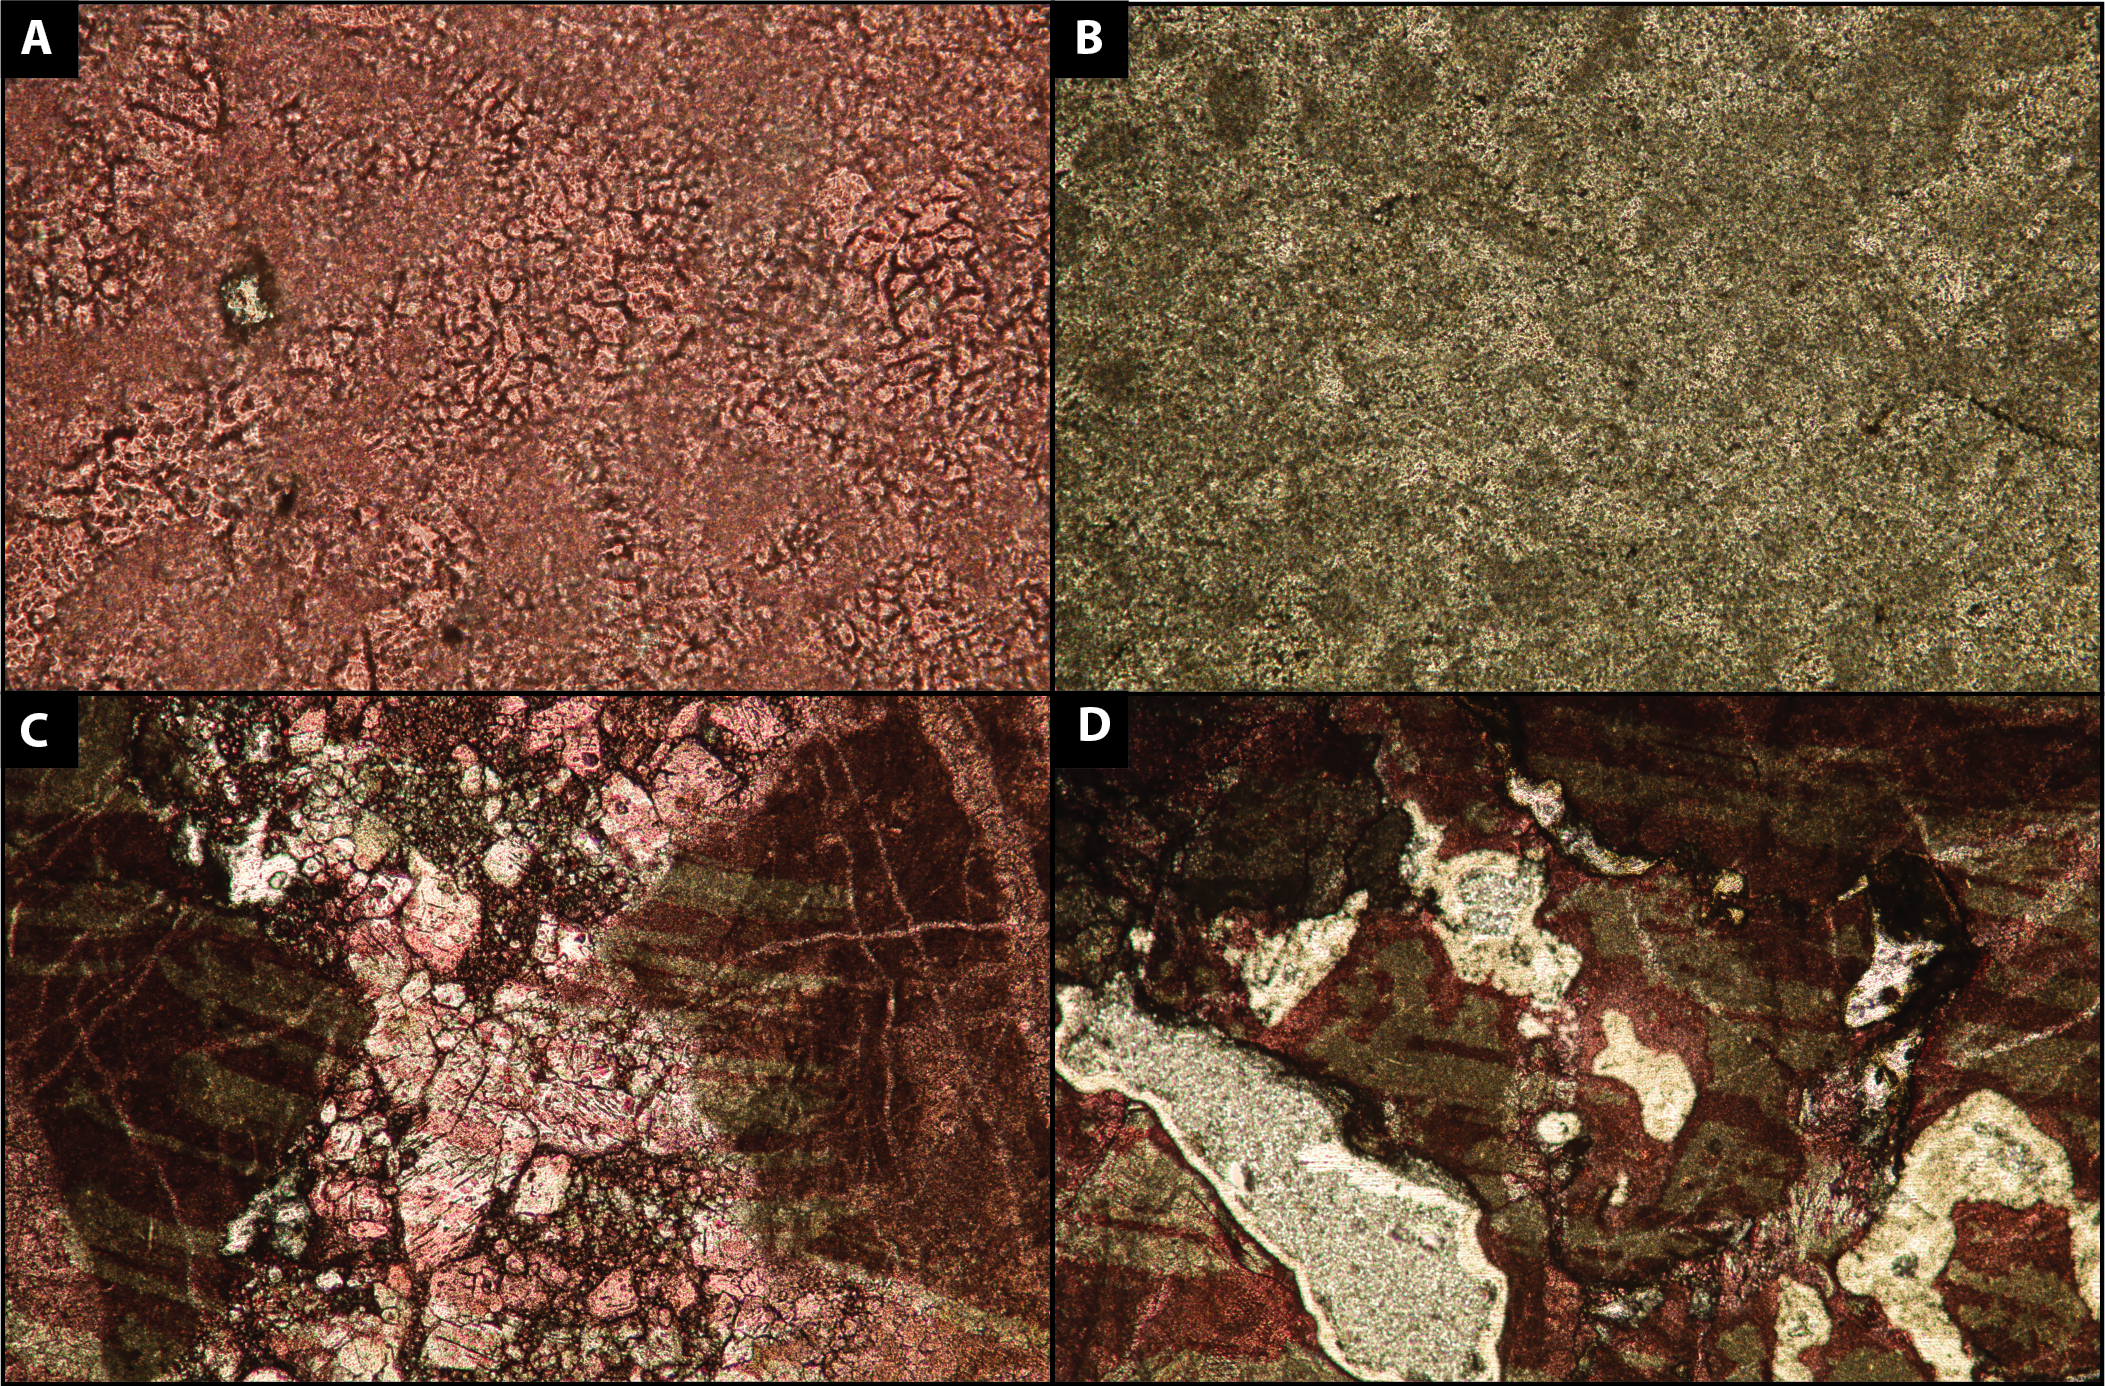
\includegraphics[width=\textwidth]{Figures/petrography/LP_thin_section_comparison.png}
    \caption{Thin sections of samples from Sch\"{o}nberg-H\"{o}hlensystem, LPSC (A\&B) and LPNS (C\&D) at 5x magnification. A) LPSC stained with alizarin red showing calcite and a single dolomite crystal. B) LPSC in PPL, showing a homogeneous micrite. C) LPNS stained for calcite. Large gray clast-like allochems and spar are visible. The staining shows some potential dolomitization. D) LPNS stained, showing void space.  }
    \vspace*{3.5in}
    \label{fig:enter-label}
\end{figure}

\subsection{Summary of Petrographic Results}

Nine samples from seven locations (Figure \ref{sitesandsamples}) were characterized by chemical and textural composition, size of allochems and matrix, solubility, and the relative percent of grains/allochems versus matrix. All well-scalloped limestones were ``pure'' (being greater than 90\% calcite)  limestones (Figure \ref{fig:dolomite-calcite-spectrum}). Sample 111123A from Parks Ranch Cave, while 83\% evaporites, was rich in Calcite. All samples are greater than 95\% soluble, with 71923A, the limestone sample from Omega Cave, being the least. Texturally, all carbonate samples except LPNS and 71923A were made of carbonate mud. LPNS is an intrasparite made of clasts of limestone or mud and calcite spar. The largest grains were found in LPNS (Table \ref{tab:petrosumary}). A summary of the petrographic results can be found in Table \ref{tab:petrosumary}. 

\newpage
\begin{figure}[t]
    \centering
    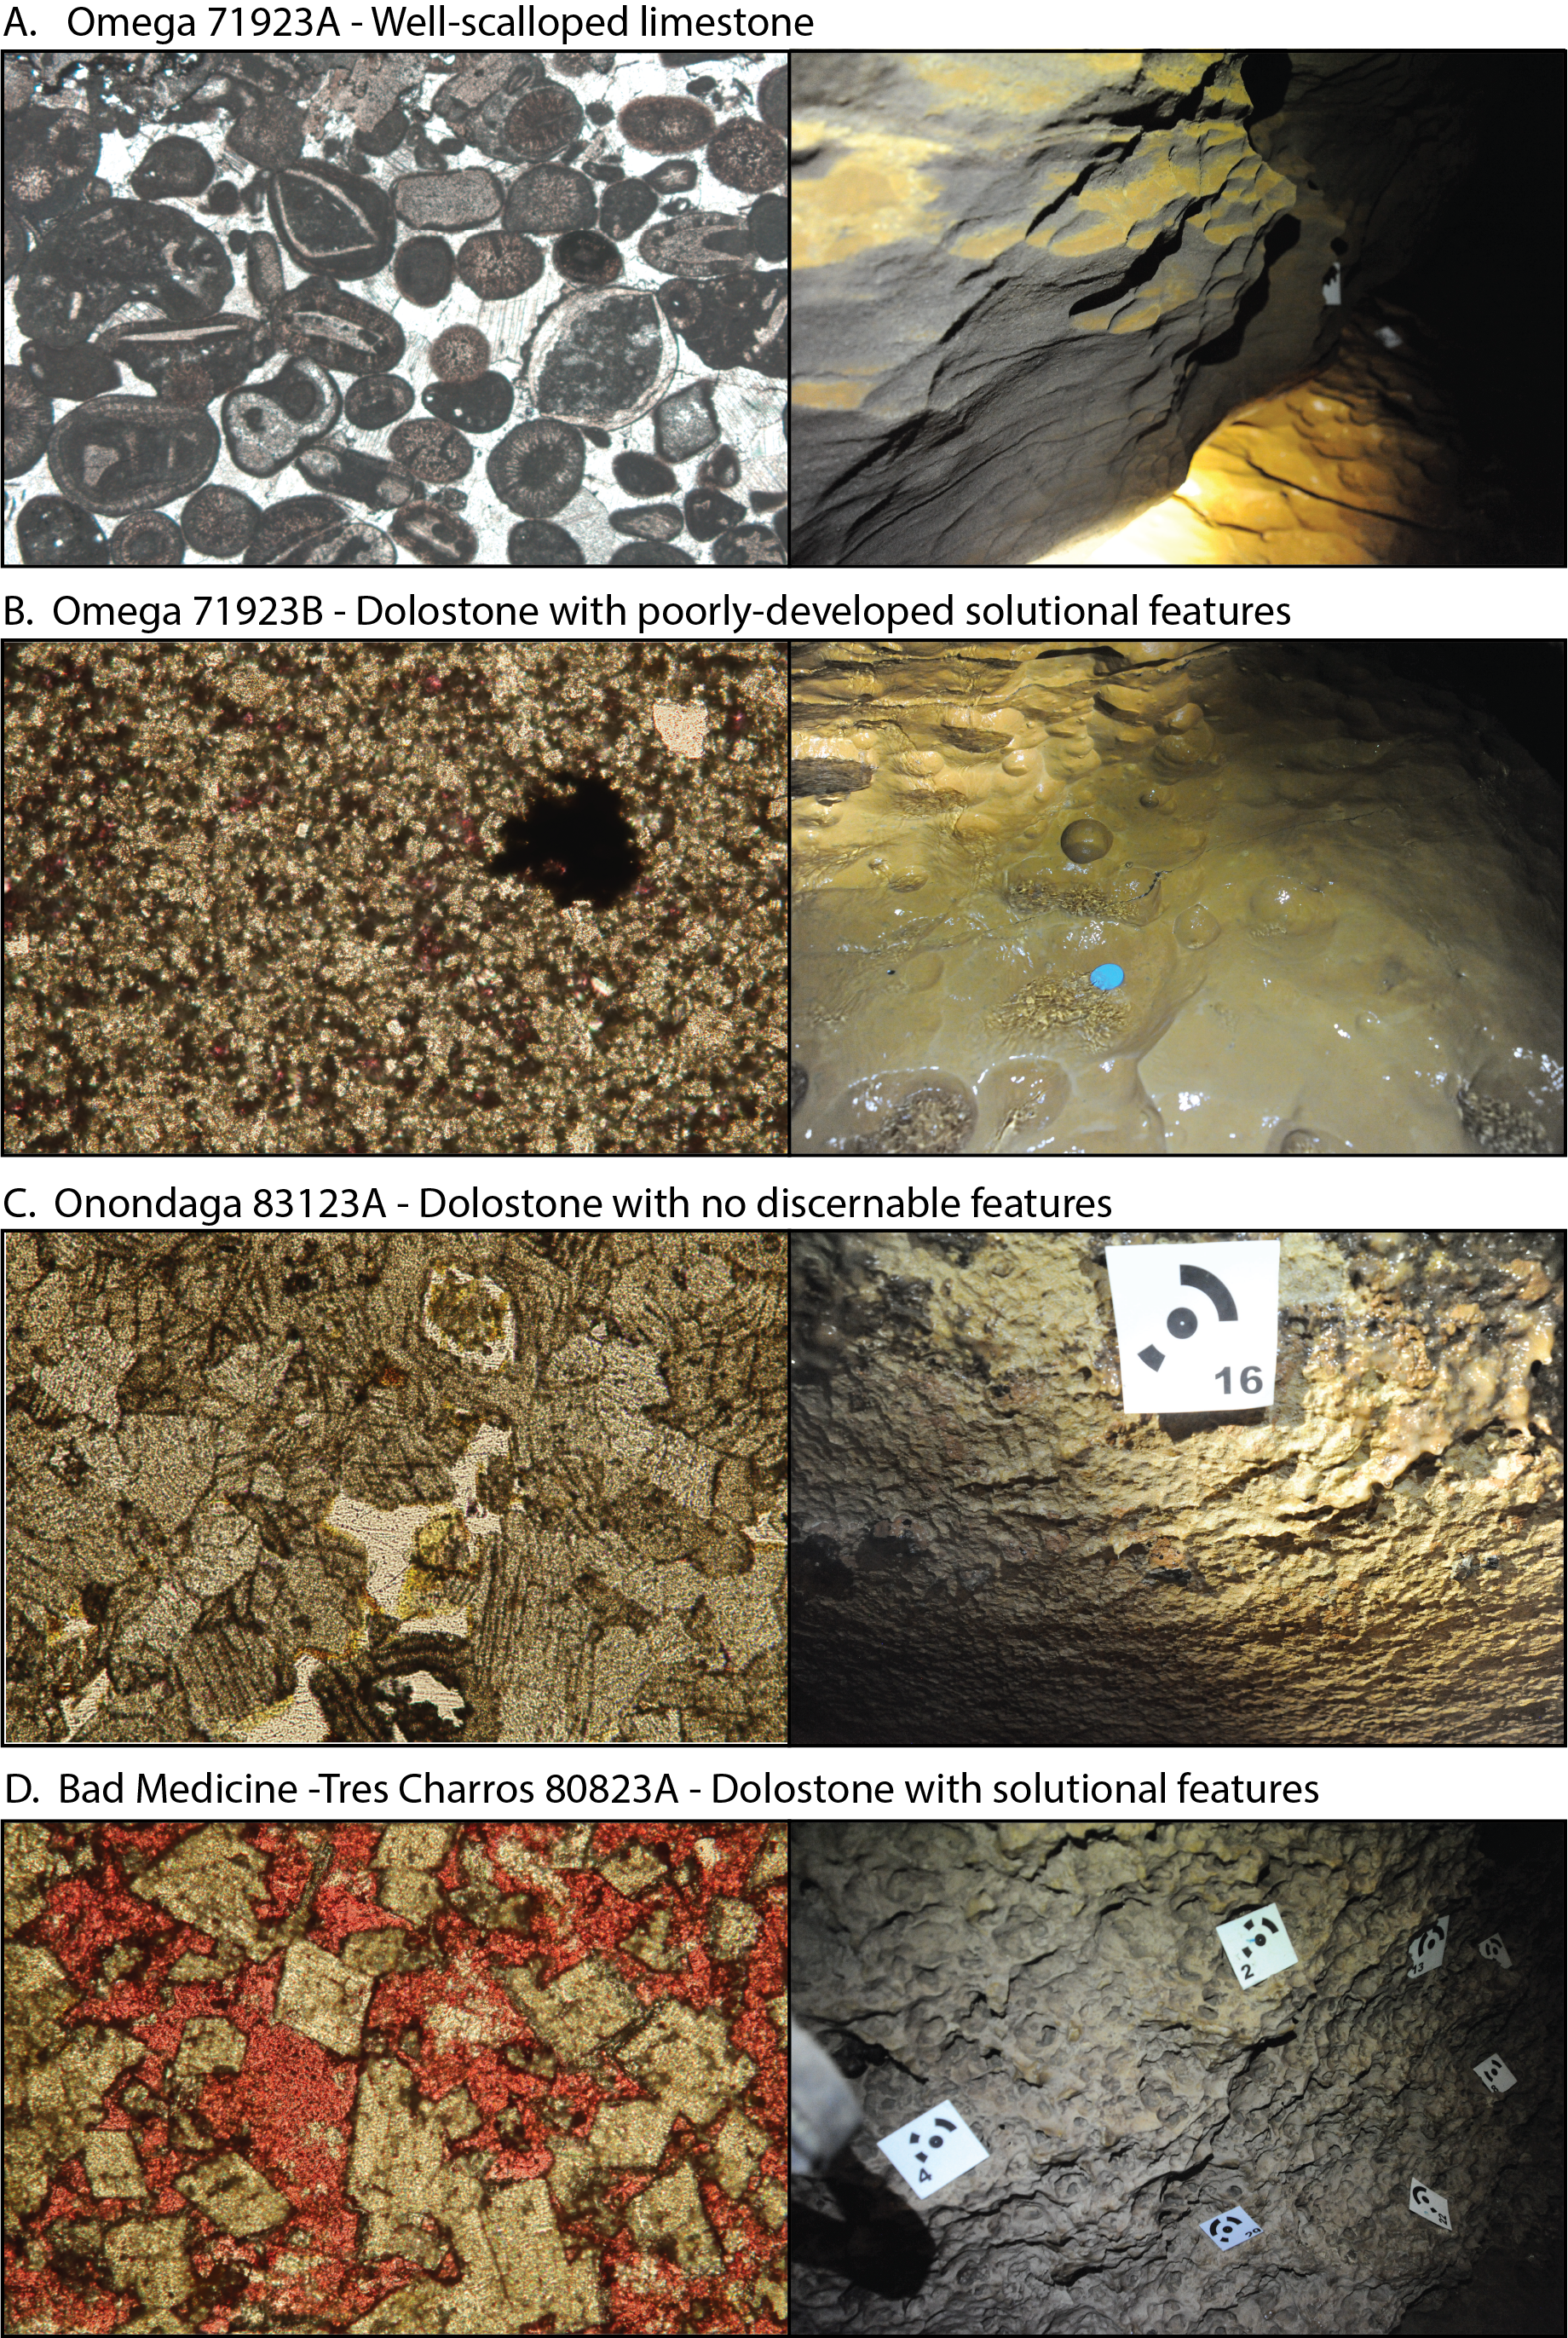
\includegraphics[scale = 0.75]{Figures/petrography/thin section and features plate 1.png}
    \caption{A representative thin section and feature for A: the Omega Limestone (71923A); B: the Omega Dolostone (71923B); C: Onondaga (83123A); and D: Bad Medicine-Tres Charros (80823A). Each site also describes the type and quality of features and chemical composition. See Table \ref{tab:petrosumary} for chemical composition and Table \ref{tab:petrosumary} for textural classification.}
    \vspace*{3in}
    \label{fig:TS and features-omega-onon-BM-TC}
\end{figure}
\newpage

\begin{figure}[t]
     \centering
     \includegraphics{Figures/petrography/resized_dolomite_spectrum.png}
     \caption{Modal composition of samples from thin section point counting. Samples with black symbols are from un-scalloped locations, while gray symbols are from scalloped locations. Note that sample 111123A from Parks Ranch Cave is not plotted as it is primarily an evaporite. Images of the features in each location can be found in Figures \ref{fig:TS and features-omega-onon-BM-TC},  \ref{fig:TS and features-BSS-PRC-j2}, and \ref{fig:TS and feature-SH}.}
     \vspace*{4.5in}
     \label{fig:dolomite-calcite-spectrum}
 \end{figure}
\newpage


\begin{figure}[t]
    \centering
    \includegraphics{Figures/petrography/violin_plots_fixed.png}
    \caption{Violin plot of grain size distributions for each sample. The white dot represents the median, the thick black line is the interquartile range, and the thin black line is the 1.5x interquartile range.  Dark gray distributions are non-scalloped, and light grey are scalloped.}
    \vspace*{4in}
    
    %{\note{I looked at the data (reported in the appendix), and there aren't any zero values. I am still messing with it, though. Do you think this is an artifact of the KDE? }}}
    \label{fig:grain_size}
\end{figure}

%\begin{landscape}
 %    \begin{table}[]
  %   \centering
   % \begin{longtable}{ | p{4cm} | p{1.5cm} | p{1.5cm} | p{1.5cm} | p{1.5cm} | p{1.5cm} | p{1.75cm} | p{1.5cm} | p{1.5cm} | p{1.7cm} |} \hline
   % \textbf{Sample} & 71923A & 71923B & 80823A & 83123A & 90423A & 111123A& J2 & LPSC & LPNS \\ \hline
   % \textbf{\% Calcite} & 95.67 & 8 & 35 & 0.67 & 99 & 14 &N/A & 90.67 & 89 \\ \hline
   % \textbf{\% Dolomite} & 0 & 91.33 & 65 & 98.67 & 1 & 0 & N/A & 9.33 & 10.67 \\ \hline
   % \textbf{\% Gypsum} & 0 & 0 & 0 & 0 & 0 & 83 & N/A & 0 & 0 \\ \hline
   % \textbf{\% Other  \dag} & 4.33 & 0.67 & 0.67 & 0.67 & 0 & 3 & N/A &0 &0.33\\ \hline
   % \textbf{Chemical\newline Composition} & LStone & DStone & Ca-rich DStone & DStone & LStone & Ca-rich Gypsum & N/A & LStone & Mg-rich Lstone \\ \hline
   % \textbf{\% Soluble} & 95.67 & 99.33 & 99.33 & 99.33 & 100 & 97 & 99.36* & 100 & 99.67 \\ \hline
   % \textbf{Folk Classification} & Om & m & m & m & Bm & N/A & Dm? & m-Dm& Is \\ \hline
   % \textbf{Mean Part Size} & 423.42 & 20.52 & 44.21 & 94.72 & 47.86 & 19.44 & 127.09 & 114.54 & 1995.75 \ddag \\ \hline
   % \textbf{Median Part Size} & 420 & 19.14 & 42.67 & 78.86 & 32.77 & 18.61 & 121.09 & 112.66 & 1839.4 \ddag \\ \hline
   % \textbf{Max, Min Part Size} & 780,\newline 150 & 39.46, \newline7.99 & 108.14, \newline 17.38 & 284.09, \newline 23.02 & 299.64, \newline12.47 & 33, \newline 10.13 & 362.9, \newline 55.84 & 191.65, \newline 42.36 &2897.66, \newline  1406.33 \ddag \\ \hline
        
    %\end{longtable}
     %\caption{Summary of petrographic results for each sample. All part sizes are in microns. Abbreviations for chemical composition: LStone-Limestone: DStone: Dolostone. Abbrviations for the Folk (1959) classification: m-micrite; s-sparite; O-Oolitic; B-Bio; D-Dis; I-intraclasts. \dag ``Other" includes percent silica and clay. * The J2 percent soluble was determined experimentally in a previous study and provided by M.D. Covington. \ddag Due to the size of the clasts, only four measurements comprise these statistics. These sizes are a minimum as some clasts were too large to measure with LAS X.}
      %\vspace*{4.5in}
     %\label{tab:petrosumary}
 %\end{table}
%\end{landscape}

\begin{landscape}

\begin{table}[]
    \includegraphics[scale=0.9]{Figures/petrography/petro_summary_table.png}
    \caption{Summary of petrographic results for each sample. All grain sizes are in microns. Abbreviations for chemical composition: LStone-Limestone: DStone: Dolostone. Abbrviations for the Folk (1959) classification: m-micrite; s-sparite; O-Oolitic; B-Bio; D-Dis; I-intraclasts. \dag ``Other" includes percent silica and clay. * The J2 percent soluble was determined experimentally in a previous study and provided by M.D. Covington. \ddag Due to the size of the clasts, only four measurements comprise these statistics. These sizes are a minimum as some clasts were too large to measure with LAS X.}
    \label{tab:petrosumary}
\end{table}
\end{landscape}

\begin{figure}[t]
    \centering
    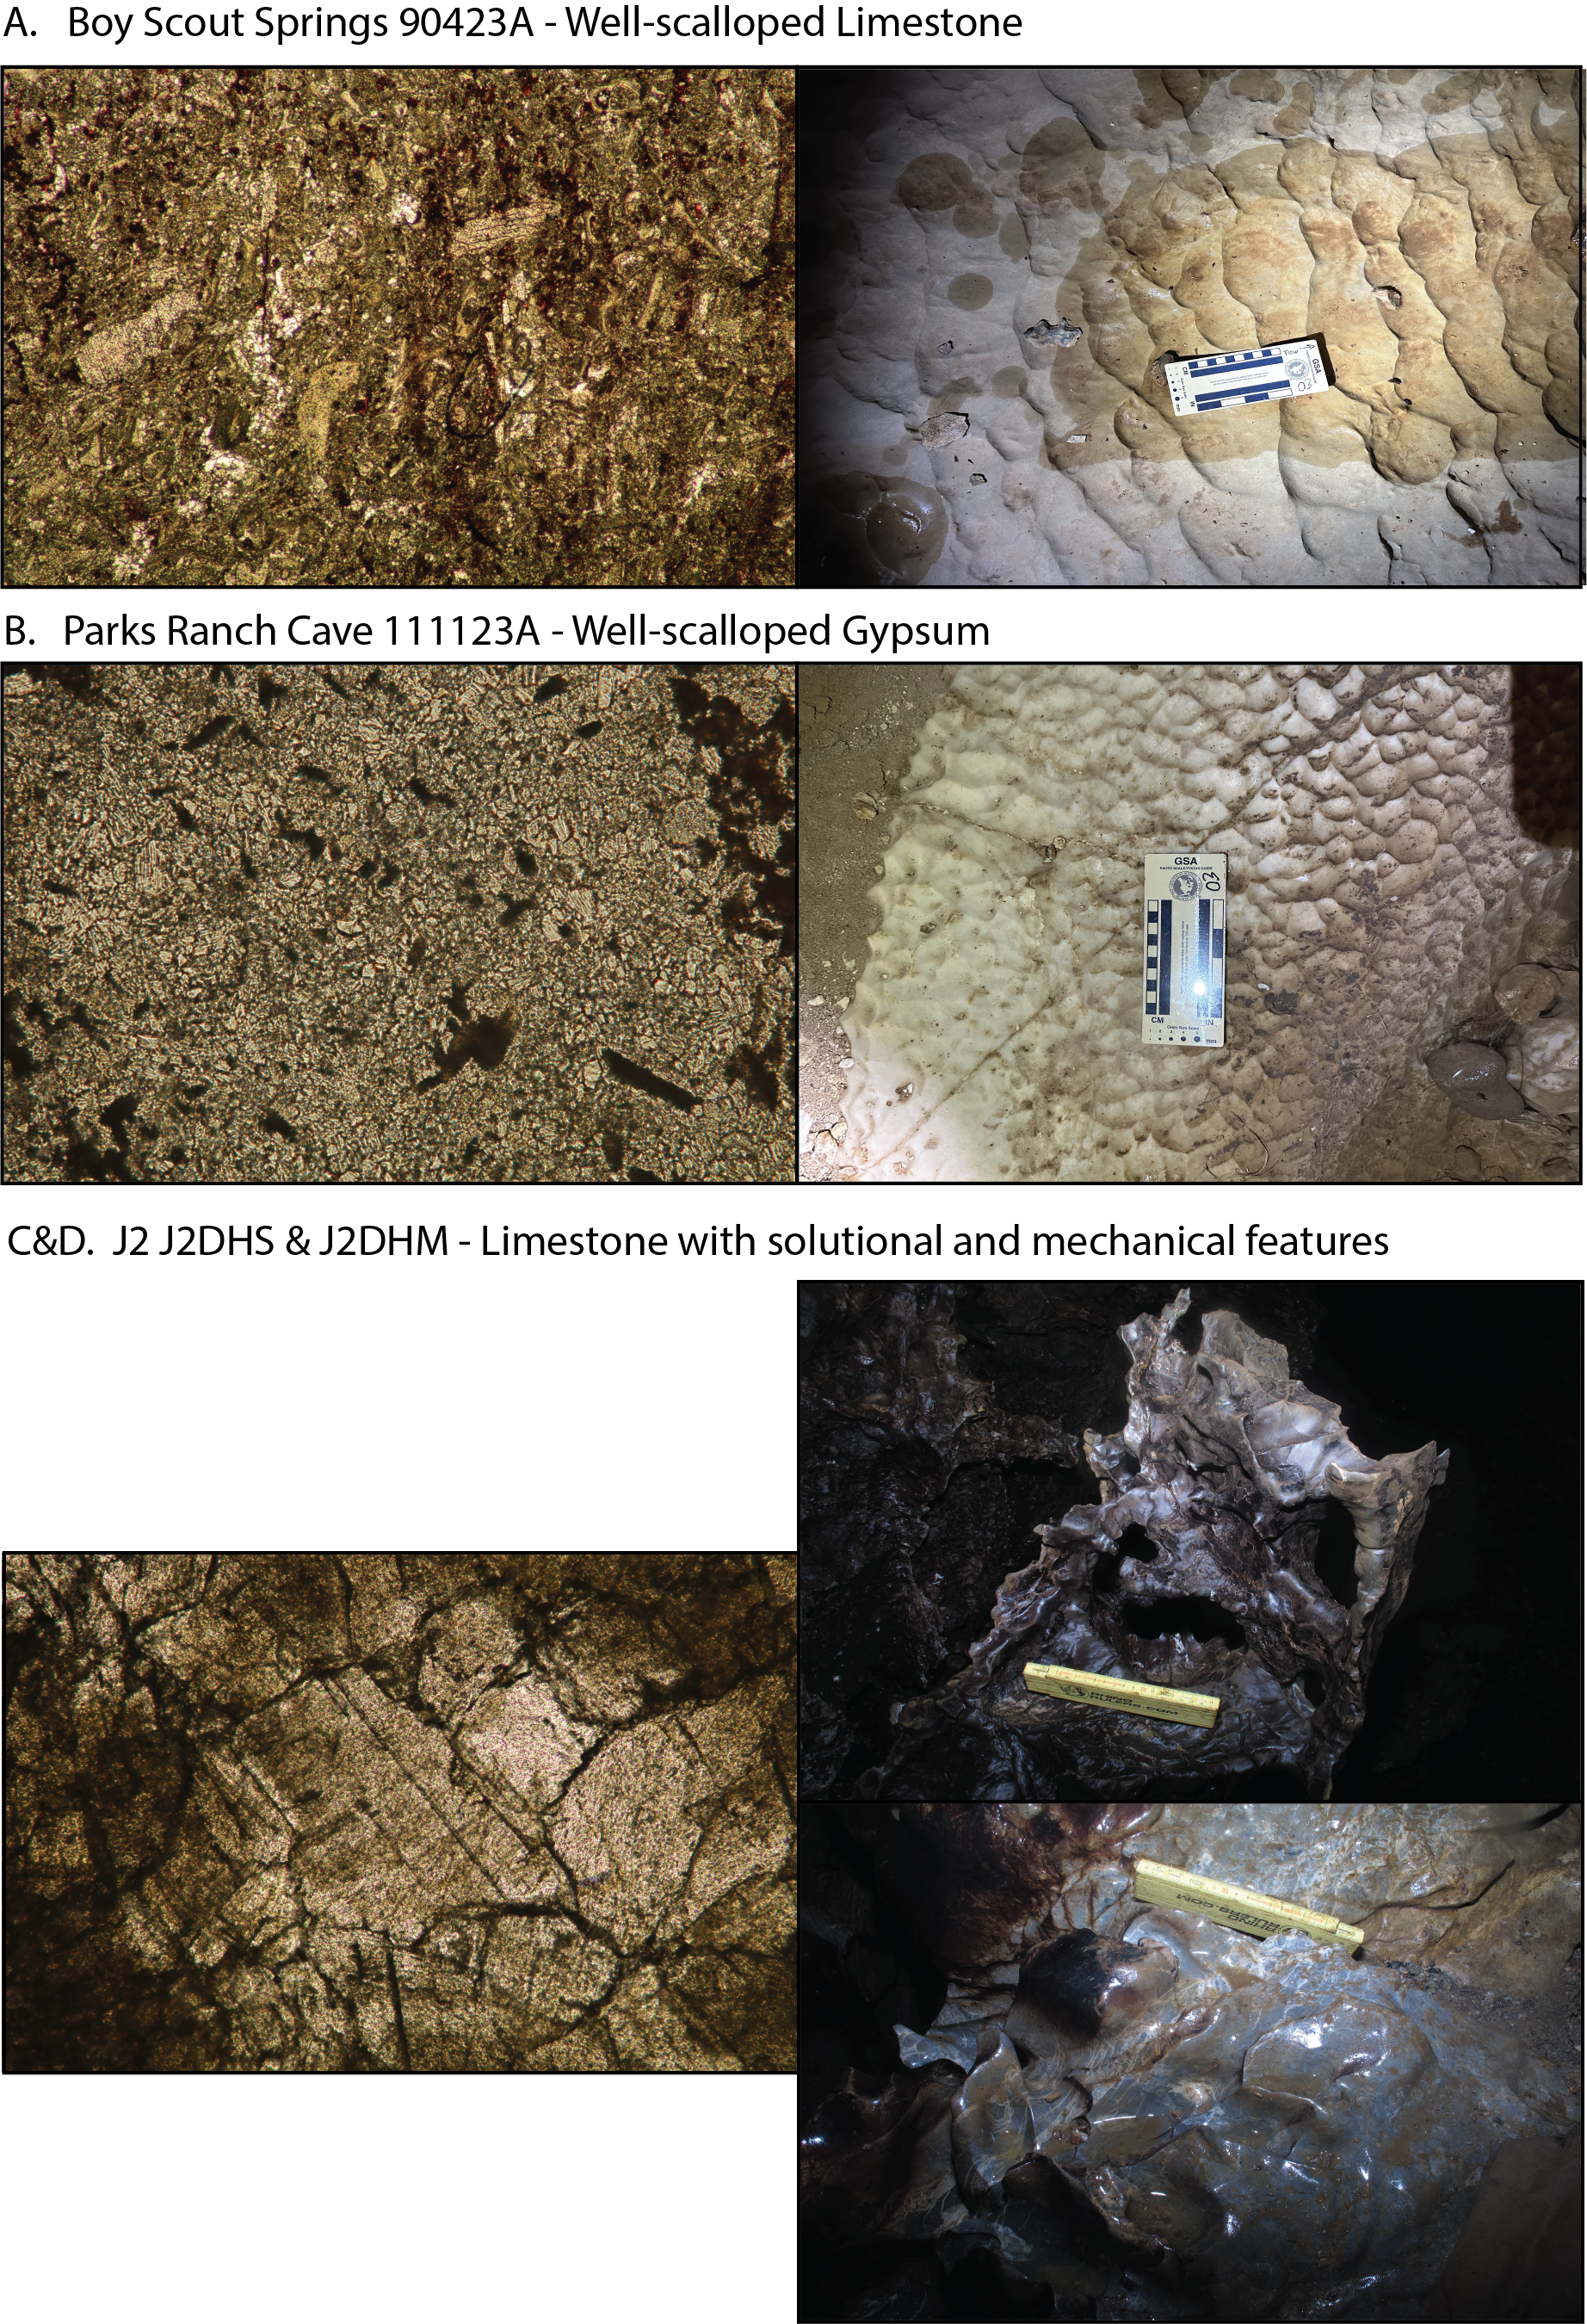
\includegraphics[scale = 0.85]{Figures/petrography/thin section and features plate 2.png}
    \caption{A representative thin section and erosional surface for A. Boy Scout Springs Cave (90423A); B: Parks Ranch Cave (111123A); and C and D: Sistema J2 (J2DHM \& J2DHS). Each site also describes the type and quality of features and chemical composition. See Table \ref{tab:petrosumary} for chemical composition and textural classification. }
     \vspace*{4.5in}
    \label{fig:TS and features-BSS-PRC-j2}
\end{figure}
\newpage
\begin{figure}[t]
    \centering
    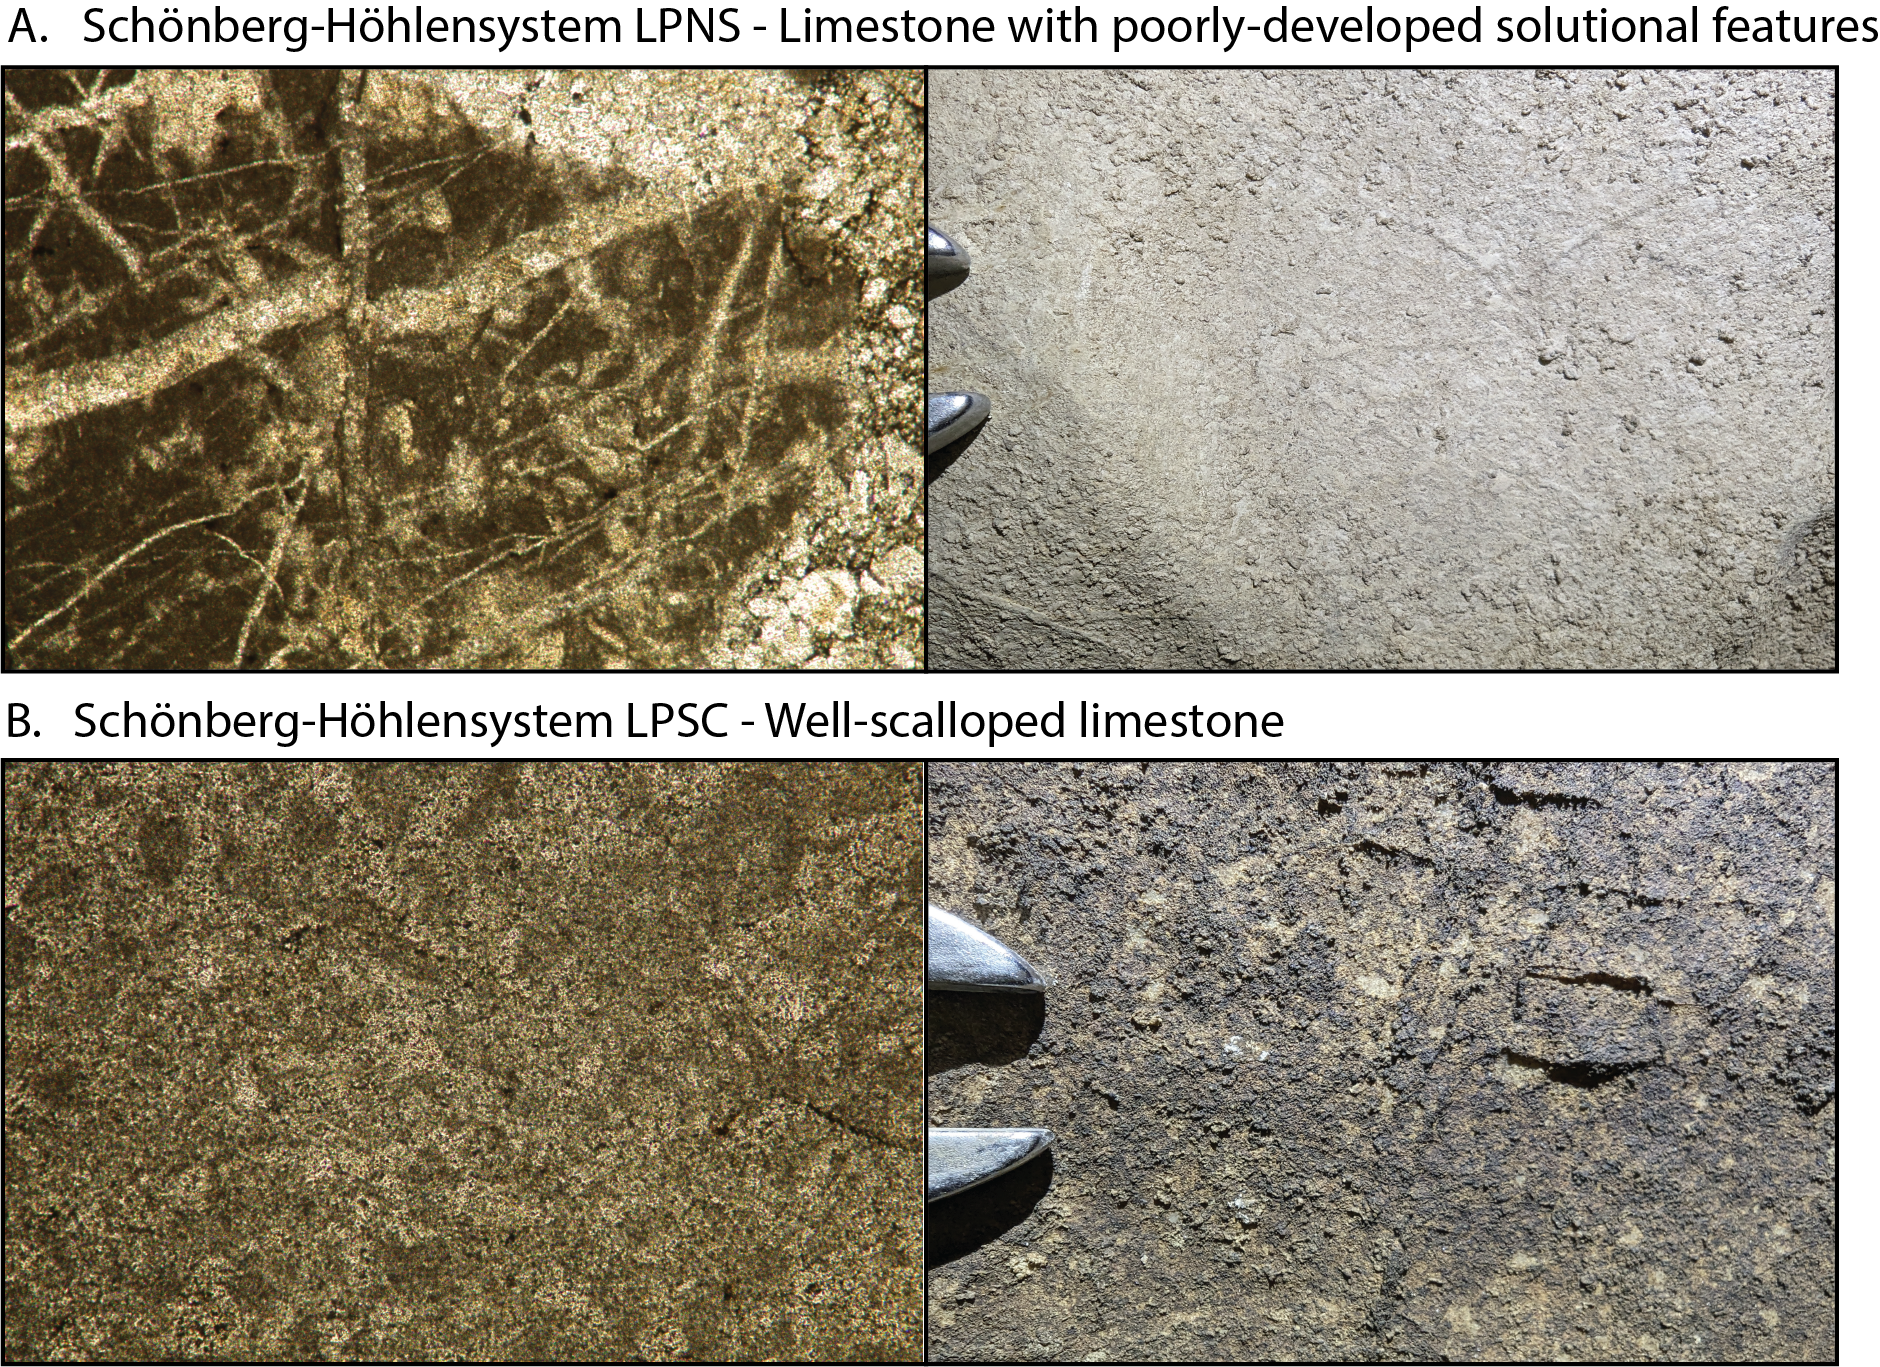
\includegraphics[scale = 0.9]{Figures/petrography/Thin section and features plate 3.png}
    \caption{A representative thin section and erosional surface for Sch\"{o}nberg-H\"{o}hlensystem samples A: LPNS and B: LPSC. The wrench in the surface photos is 13mm. Each site also describes the type and quality of features and chemical composition. See Table \ref{tab:petrosumary} for chemical composition and Table \ref{tab:petrosumary} for textural classification.}
     \vspace*{4.5in}
    \label{fig:TS and feature-SH}
\end{figure} 
\newpage





%\begin{table}[h!]
 %   \centering
  %      \begin{longtable}{p{1.5cm} | p{2cm} p{1.5cm}  p{1.5cm} p{1.5cm} p{1.5cm}} \\
   %     \textbf{Sample} & \textbf{Cave} &  \textbf{Mean} & \textbf{Median}& \textbf{Max} &\textbf{ Min} \\ \hline

   %     71923A & Omega & 423.42 & 420 & 780 & 150 \\ 
   %     79123B & Omega & 20.52 & 19.14 & 39.46 & 7.99 \\ 
   %     80823A & BM-TC & 44.21 & 42.67 &108.14 & 17.83 \\ 
   %      83123A & Onondaga & 94.72 & 78.86& 284.09 & 23.02 \\ 
   %     90423A &BSS & 47.86 &  32.77 & 299.64  & 12.47 \\
   %     111123A & PRC&  19.44 & 18.61 & 33 & 10.13 \\ 
   %     J2*  & Sistma J2 & 127.09 & 121.09 & 362.92 & 55.84 \\ 
   %     LPSC & SH& 114.54 & 112.66&  191.65 & 42.36 \\ 
   %     LPNS & SH& 174.36 & 138.68 & 726.002 & 49.39 \\         
%  \end{longtable}
   % \caption{Descriptive statistics for size analysis of constituent parts showing mean, median, max, and min in microns. *Samples J2DHS and J2DHM share one thin section. BM-TC- Bad Medicine-Tres Charros; PRC - Parks Ranch Cave; SH - Sch\"{o}nberg-H\"{o}hlensystem; BSS - Boy Scout Springs Cave. }
   % \label{tab:grain_sizes}
%\end{table}

%\begin{table}[h!]
 %   \centering
 %  \begin{longtable}{p{1.5cm} | p{2.3cm}  p{2.5cm}  p{2.3cm}  p{2.3cm} p{2.5cm} }
%\textbf{Sample} & \textbf{\% Calcite} & \textbf{\% Dolomite} & \textbf{\% Gypsum} & \textbf{\% Other} & \textbf{Chemical \newline Classification} \\ \hline

%71923A & 95.67 & 0 & 0 & 4.33 & Limestone \\ 
%71923B & 8 & 91.33 & 0 & 0.67 & Dolostone \\
%80823A & 0 &  99.33 & 0 & 0.67 & Dolostone \\
%83123A & 0.67 & 98.67 & 0 & 0.67 & Dolostone \\
%90423A & 99 & 1 & 0 & 0 & Limestone \\
%111123A & 14 & 0 & 83  & 3 & Gypsum \\
%LPSC & 90.67 & 9.33 & 0 & 0& Limestone \\
%LPNS & 89 & 10.67 & 0 & 0.33 & Mg-rich Limestone \\


%\end{longtable}   
 %  \caption{Compositions of sample rocks from point counting. The percentage of ``other'' includes percent silica and percent clay. }
%\label{tab:chemical_comp_of_thin_sections}
%\end{table}

% Table order (going down): 71923A, 71923B, 80823A, 83123A, 90423A, 111123A, J2, LPNS, LPSC

%\begin{table}[]
%  \centering
 %   \begin{longtable}{p{2cm} p{2cm} p{2cm}}
  %  \textbf{Sample} & \% Grains & \% Matrix \\ \hline
  
   % 71923A & 68 & 32 \\
   % 71923B & 68 & 32 \\
   % 80823A & 49 & 51 \\
   % 83123A & 88 & 12 \\
   % 111123A & 85 & 15 \\
   % 90423A & 78 & 22 \\
   % J2 & 56 & 44 \\
   % LPSC & 80 & 20 \\
   % LPNS & 85 & 15 \\
    
   % \end{longtable}
   % \caption{Caption}
%\label{tab:Modal_comps}
%\end{table}
\newpage


\section{ESEM}

Environmental Scanning Electron Microscopy, or ESEM, produced high-resolution, \\ monochromatic images of the sample surface. All samples were imaged from ~30x to 1000x. The samples from scalloped sites: Omega (71923A), Boy Scout Springs (90423A), and Parks Ranch Cave (111123A), were imaged on their scalloped surface. Other solutional features were imaged in an area of the sample that was representative of the features present. Mechanically eroded samples were also imaged in this way. Panels of ESEM images for each sample can be found in Figures \ref{fig:ESEM-omega-bmtc-bss-prc}, \ref{fig:j2_comp}, and \ref{fig:esem-lpsc-lpns}. 


\subsection{Omega}
\subsubsection{71923A}
71923A is a scalloped limestone from Omega Cave. This sample is an oomicrite (Table \ref{tab:petrosumary}). The ESEM image (Figure \ref{fig:ESEM-omega-bmtc-bss-prc})  taken at  50x magnification as well as the image taken at 38x (Figure \ref{fig:omega_at_38_x}) show spherical grains held in a finer groundmass. The larger grains are within the size range (~0.5 mm) of the ooids from the 71923A thin section (Figure \ref{fig:TS and features-omega-onon-BM-TC}). The 50x image also shows some localized pitting. Zooming in on these pits (Figure \ref{fig:ESEM-omega-bmtc-bss-prc}), they appear to be 100s of microns wide and 10s of microns deep (inferred from contrast and pit walls). The pits appear to lack a consistent geometry. Within the 50x image (Figure \ref{fig:ESEM-omega-bmtc-bss-prc}), there appears to be a ``micro-scallop” pattern that follows the flow directionality of the larger scallop where downstream is to the upper right of the image. The micro-scallops are on the order of 100s of microns in length. 

\subsection{Bad Medicine-Tres Charros}
80823A is an un-scalloped, solutional feature in a dolostone micrite. The images of 80823A at 50x (Figure \ref{fig:TS and features-omega-onon-BM-TC}) show a relatively homogeneous surface without any noticeable patterns or mechanical tool marks. The surface appears to have high relief, inferred from the color contrast. Throughout the surface, pits are noticeable. These pits are clearer in Figure \ref{fig:BM_TC_at_30x}, taken at 30x. They are on the order of 100s of microns in length. Closely looking at these pits in Figure \ref{fig:TS and features-omega-onon-BM-TC}, the geometry of the perimeter is polygonal, and some of the surrounding grains appear to be close to detachment. 



\subsection{Boy Scout Springs}
Sample 83123A is a scalloped sample of biomicrite. The surface of the scallop (Figure \ref{fig:TS and features-omega-onon-BM-TC}) shows tool marks throughout the sample. These tool marks are several 100s of microns long and 10s of microns wide. The more prominent marks are oriented to the image's lower left. Figure \ref{fig:TS and features-omega-onon-BM-TC} shows two tool marks at ~100x magnification. The surface of the scallop is otherwise of low relief, and several areas appear to be almost smooth. 

\subsection{Parks Ranch Cave}
The images (Figure \ref{fig:TS and features-omega-onon-BM-TC}) of a scallop from Parks Ranch Cave, sample 111123A, show a surface with a complex relief. There are several pits on the surface, but no pattern overall.  The pits have no distinguishable geometry and are lined with more fibrous anhydrite grains (Figure \ref{fig:TS and features-omega-onon-BM-TC}). At 1000x, the individual gypsum crystals are visible (Figure \ref{fig:parc_1000x}).


\subsection{Sistema J2}
\subsubsection{J2DHS}
J2DHS, a solutional, non-scalloped sample from Sistema J2, imaged at 250x, shows a surface with high relief and complexity (Figure \ref{fig:j2_comp}). There is no overall pattern, and several pits are present. The pits lack a consistent geometry.

\subsubsection{J2DHM}
The surface of the mechanically eroded J2DHM has low relief and low complexity (Figure \ref{fig:j2_comp}). It is markedly different from its solutional mate, J2DHS. A smooth coating appears across the surface, preserving abrasion tool marks. When the actual surface is shown, it also has low relief. The tool marks are microns wide, but in some cases, traverse the whole surface (Figure \ref{fig:j2DHM}). There are two major orientations of the marks (Figure \ref{fig:j2_comp}) that cross each other and point to the corners of the image in Figure \ref{fig:j2DHM}. 



\subsection{Sch\"{o}nberg-H\"{o}hlensystem}
\subsubsection{LPSC}
The scalloped LPSC is oriented in Figure \ref{fig:esem-lpsc-lpns} so that the downstream direction is to the upper right corner of the image. Though faint, there appears to be a pattern parallel to the downstream direction not too dissimilar from that of the ``micro-scallop” pattern of 71923A. The scalloped surface shows high relief and moderate complexity, with local high spots in the topography (Figure \ref{fig:esem-lpsc-lpns}). No indications of mechanical processes, such as tool marks, are present. 

\subsubsection{LPNS}
LPNS is a non-scalloped intrasparite with no indications of well-formed features. The surface of this sample is high relief, with localized pitting that appears deep (Figure \ref{fig:esem-lpsc-lpns}). The surface has no regular pattern and is of high complexity. The deep pits do not have a pattern, though they appear to contain detritus from the sample (Figure \ref{fig:esem-lpsc-lpns}).

\subsection{Summary of ESEM Results} 
The ESEM images taken of the sample surface provide high-resolution, qualitative descriptions of each sample and the differences between mechanical and solutional features and those in between. The solutional and scalloped surfaces (71923A, 80823A, 90423A, 111123A, J2DHS, LPSC, and LPNS) appear to be higher relief, higher complexity, and with no pattern to surface marks. On two scalloped samples, 71923A and LPSC, there is a weak pattern of ``micro-scallops,” which mirrors the directionality of the larger feature. The mechanical samples, J2DHM and, to some extent, 90423A, show clear signs of mechanical erosion processes, such as tool marks. Samples 90423A and 80823A from Bad Medicine-Tres Charros exhibit the characteristics of both the mechanical and solutional features. 

\begin{figure}[t]
    \centering
    \includegraphics[scale=0.85]{Figures/ESEM/ESEM Panel 1 - omega-BMTC-BSS-PRC.png}
    \caption{ESEM images of A \& B: Omega Cave Limestone (71923A); C \& D: Bad Medicine-Tres Charros; E \& F:Boy Scout Springs Cave; and G \& F: Parks Ranch Cave with scale bars and magnification.}
     \vspace*{4.5in}
    \label{fig:ESEM-omega-bmtc-bss-prc}
\end{figure}

\begin{figure}[t]
    \centering
    \includegraphics[scale=0.9]{Figures/ESEM/j2_ESEM_compare.png}
    \caption{ESEM images of the two samples from Sistema J2: J2DHM (top) and J2DHS (bottom). Tool marks are visible in J2DHM. The image of J2DHS shows a pit surrounded by a complex and high-relief surface. }
     \vspace*{4.5in}
    \label{fig:j2_comp}
\end{figure}

\begin{figure}[t]
    \centering
    \includegraphics[width = \textwidth]{Figures/ESEM/ESEM Panel 2-LPSC and LPNS.png}
    \caption{ESEM images of samples from Sch\"{o}nberg-H\"{o}hlensystem: A \& B: LPSC sand C \& D: LPNS with scale bars and magnifications. The surface of LPSC is homogeneous and high relief. The surface of LPNS is locally pitted, high relief, and heterogeneous. }
     \vspace*{4.5in}
    \label{fig:esem-lpsc-lpns}
\end{figure}


\begin{figure}[t]
    \centering
    \includegraphics[width=\textwidth]{Figures/ESEM/5.jpeg}
    \caption{ESEM image of 71923A from Omega Cave at 38x magnification. There are noticeable spheres on the surface that are likely ooids. }
     \vspace*{4.5in}
    \label{fig:omega_at_38_x}
\end{figure}


\begin{figure}[t]
    \centering
    \includegraphics[width=\textwidth]{Figures/ESEM/PIC13.jpeg}
    \caption{An image of the sample from Bad Medicine-Tres Charros showing pits on the surface of the solutional feature. The pits are 100s of microns in length.}
     \vspace*{4.5in}
    \label{fig:BM_TC_at_30x}
\end{figure}

\begin{figure}[t]
    \centering
    \includegraphics[width = \textwidth]{Figures/ESEM/10.jpeg}
    \caption{ESEM image of a scallop from Parks Ranch Cave at 1000x showing individual gypsum grains.}
     \vspace*{4.5in}
    \label{fig:parc_1000x}
\end{figure}

\begin{figure}[t]
    \centering
    \includegraphics[width = \textwidth]{Figures/ESEM/1.jpeg}
    \caption{Surface of J2DHM showing a low relief surface with mechanical took marks in two orientations.}
     \vspace*{4.5in}
    \label{fig:j2DHM}
\end{figure}


\section{Confocal Roughness}

The roughness, measured by confocal microscopy, was calculated for mechanical-solutional pairs (Omega and Sistema J2) and samples from Sch\"{o}nberg-H\"{o}hlensystem. The solutional samples from Sistema J2 and Omega had a higher surface roughness than their mechanical pair. Both samples were taken in identical locations in the stratigraphic column in their respective cave. The main confocal microscopy results are the mean surface height, $Sa$, and the area-scale fractal complexity, $Asfc$, values (Table \ref{tab:confocal_table}). For the results section $Asfc$ can be thought of as a a change in roughness with respect to the scale of calculation. 

In the case of the samples from Sistema J2, the solutional surface was 20x rougher ($Sa = 27.03\ \mu m$) than the mechanical surface ($ Sa = 1.33\ \mu m$). This significant difference in roughness is visible not only in the ESEM images (Figure \ref{fig:j2_comp}) but also in the 3D models and surface maps rendered from the confocal data (Figures \ref{fig:roughness_map_of_J2DHM}, \ref{fig:roughness_map_of_J2DHS}, and \ref{fig:3D j2DHMl}). Asfc shows an even more significant disparity where the solutional surface has a $\sim$ 30x greater change in roughness. The roughness of the solutional sample (71923BSolo) from Omega Cave was $13.71 \ \mu m$, while the mechanical sample (71923BMech) was less rough at $7.26\ \mu m$. Compared to the Sistema J2 samples, the Omega samples exhibit the same higher surface roughness for the solutional surface but display the opposite case for Asfc. The solutional surface from Sistema J2 (J2DHS) had a high $Asfc$, but the mechanical surface (J2DHM) had a much lower $Asfc$ (Table \ref{tab:confocal_table}). While the solutional surface has more relief than the mechanical surface, the change in roughness, akin to a roughness gradient, is less. 

The pair from Sch\"{o}nberg-H\"{o}hlensystem exhibit a high relief and a high roughness gradient. LPSC, the scalloped sample, has a similar roughness to the other scalloped samples (Figure \ref{fig:Sa_v_cave}), though comparing samples from different sites may be problematic. The non-scalloped feature, LPNS, has a relief and a roughness gradient within the same order of magnitude as LPSC. LPNS, as supported by Figure \ref{fig:schon_pic}, may have solutional features but not scallops. 

%Sample 111123PRC1, from Parks Ranch Cave, a sample with well-formed scallops, had a roughness of $4.680 \mu m$, and a change in roughness of $8.440 \mu m$. There is no comparative mechanical feature for Parks Ranch Cave. The roughness is within the same order of magnitude of the mechanical features from both Omega and Sistema J2. 

\begin{table}[t]
  \includegraphics[width=\textwidth]{Figures/Roughness/confocal_results.png}
    \caption{Results of Confocal roughness analysis. For true mechanical-solutional pairs (samples from Omega and J2), the solutional surfaces have higher relief $(Sa)$ than their mechanical mate. SH: Sch\"{o}nberg-H\"{o}hlensystem, J2: Sistema J2.}
   \label{tab:confocal_table}
\end{table}

\begin{figure}[t]
    \centering
    \includegraphics[scale = 0.5]{Figures/Roughness/j2mech_map.jpeg}
    \caption{Surface map of J2DHM, the mechanical sample from Sistema J2. Tool marks from abrasion are visible. The mean roughness of this sample is 1.33 $\mu m$. Scale bar is in microns, x and y axes in mm.}
    \vspace*{4.5in}
    \label{fig:roughness_map_of_J2DHM}
\end{figure}

\begin{figure}[t]
    \centering
    \includegraphics[scale = 0.5]{Figures/Roughness/omega_solo_map.jpeg}
    \caption{Surface Map of 71923BSolo, the solutional sample from Omega Cave. The mean roughness of this sample is 13.71 $\mu m$. Scale bar is in microns, x and y axes in mm.}
     \vspace*{4.5in}
    \label{fig:roughness_map_of_J2DHS}
\end{figure}

\begin{figure}[t]
    \centering
    \includegraphics[width =\textwidth]{Figures/Roughness/fixed_roughness.png}
    \caption{Surface roughness, Sa (in microns), and Area-scale fractal complexity, Afsc, by cave showing feature type. Error for these measurements is $\pm 0.2\ \mu m$. The error bars are not visible when plotted.}
     \vspace*{4.5in}
    \label{fig:Sa_v_cave}
\end{figure}


\begin{figure}[t]
    \centering
    \includegraphics[scale = 0.5]{Figures/Roughness/lpsc_map.jpeg}
    \caption{Surface map of LPSC, the scalloped sample from Sch\"{o}nberg-H\"{o}hlensystem. The mean roughness of LPSC is 12.51 $\mu m$. Scale bar is in microns, x and y axes in mm.}
    \vspace*{4.5in}
    \label{fig:roughness_map_of_LPSC}
\end{figure}

\begin{figure}[t]
    \centering
    \includegraphics[scale = 0.5]{Figures/Roughness/lpns_map.jpeg}
    \caption{Surface map of LPNS, the non-scalloped sample from Sch\"{o}nberg-H\"{o}hlensystem. The mean roughness of LPNS is 20.35 $\mu m$. Scale bar is in microns, x and y axes in mm.}
    \vspace*{4.5in}
    \label{fig:roughness_map_of_LPNS}
\end{figure}


\section{Scallop Geometry Results}

Three of the five sites visited had well-formed scallops measured: Boy Scout Springs Cave, Parks Ranch Cave, and Omega Cave. At each site, several hundred photos of the passage and scallops were taken, and of those pictures, 30-40 well-formed, clear scallops were measured. The features present, the distribution of scallop lengths, their means, and their aspect ratio will be described for each location. Means will be reported using both arithmetic and Sauter values. The Sauter mean gives greater weight to larger values and is traditionally the method of reporting scallop lengths \citep{curl, springerandwohl, springerandhall}. The Sauter mean is calculated by the following equation: 
\begin{equation}
    \overline{L_{32}} = \frac{\Sigma l^{3}_{i}}{\Sigma l^{2}_{i}}
\end{equation}\label{sauter}
where, $L_{32}$ is the Sauter mean and $l_i$ is the $ith$ scallop \citep{curl}. Alongside the descriptive statistics, the Shapiro-Wilk test for normality is calculated \citep{springerandhall}. The Shapiro-Wilk statistic tests the hypothesis that the sample is from a normal distribution. A value of 1.0 indicates an ideal, normal distribution. In this study, the threshold for significance is 0.05. This value for significance is common but also used in other scallop literature \citep{springerandhall}. 

\subsection{Boy Scout Springs}

The sampled passage in Boy Scout Springs is at the active stream level. It is low but wide, with large deposits of sediment ranging from clay to cobble in size present (Figure \ref{fig:BSS-passage}). The measured scallops were mostly on the floor of the passage and, thus, are likely the largest (being formed by the slowest flows in normal conditions). The distribution of scallop lengths (Figure \ref{fig:scallop-length-histo}) was calculated from 38 scallops. The Sauter mean, which provides greater weight to larger values, is 6.19 cm, and the arithmetic mean is 4.45 cm. The mean aspect ratio of the scallops is 0.92 (Equation \ref{eq:sphere}). The results of the Shapiro-Wilk test for normality show that the scallop lengths for Boy Scout Springs are likely not from a normally distributed population with a test statistic of 0.95, but a p-value of 0.08 (Table \ref{tab:scallop_lengths_stats}). 

\begin{figure}[t]
    \centering
    \includegraphics[scale=0.09]{Figures/pictures/IMG_0526.jpeg}
    \caption{Sample location in Boy Scout Springs Cave, AR. The passage is wide and low. Most scallops are on the floor. Sediment deposits in the passage contain clay to cobble-sized particles.}
    \vspace*{4.5in}
    \label{fig:BSS-passage}
\end{figure}

\subsection{Parks Ranch Cave}

Parks Ranch Cave, a multi-level gypsum cave was sampled in a lower passage with pooled water, but not the active stream. The scallop length decreases closer to the ceiling \citep{nance} to the sub-centimeter scale. Descriptive statistics were calculated from 39 scallops (Figure \ref{fig:scallop-length-histo}). The scallops of Parks Ranch Cave comprise the smallest measured features with a Sauter mean of 3.25 cm and an arithmetic mean of 2.79 cm. The mean aspect ratio was 1.08 (Table \ref{tab:scallop_lengths_stats}). The distribution is the most normal of the histogram, and it has a Shapiro-Wilk statistic of 0.97, where a value of 1.0 is ideal, and a p-value of 0.26. Therefore, whether this sample is from a normally distributed population is uncertain. 

\subsection{Omega Cave}
The scallops in Omega Cave were measured at the base level of the cave in the active stream passage. The scallops are on the walls of the passage in limestone (79123A), while the floor is made of dolostone (71923B). The scallop statistics were calculated from 30 scallops from the wall. The Sauter mean for this population is 10.04 cm, while the arithmetic mean is 5.57cm. The mean aspect ratio is 1.05 (Table \ref{tab:scallop_lengths_stats}). This population is clearly not normal, with a strong right skew (Figure \ref{fig:scallop-length-histo}). The Shapiro-Wilk test underscores the non-normality of this distribution with a test statistic of 0.86 and a p-value of 0.00092. 

\subsection{Non-scalloped features}
At each site, several feature types were observed (Table \ref{tab:features_per_sites}). The most common feature, besides scallops, were solution pockets. Solution pockets differ from scallops in that they are symmetrical, usually deeper, discrete, and often aligned with fractures \citep{springerandwohl, palmercavegeo}. Other features observed were mechanical flutes and potholes formed by abrasion. The features found in Bad Medicine-Tres Charros, colloquially known as ``velcro", have the appearance of solutional features but are listed in Table \ref{tab:features_per_sites} as chemomechanical due to observations from ESEM (Figure \ref{fig:BM_TC_at_30x}). 

\newpage

\begin{figure}[]
    \centering
    \includegraphics[scale = .78]{Figures/Scallop Lengths/fixed_measurements.png}
    \caption{Histograms of the downstream length, $l$, and aspect ratio (Equation \ref{eq:sphere}) of scallops in Boy Scout Springs Cave, Parks Ranch Cave, and Omega Cave. The aspect ratio distribution and its mean are shown in the right column for each sample. Shapiro-Wilk test for normality results for each scallop length distribution, arithmetic mean and Sauter mean, and aspect ratio are shown in Table \ref{tab:scallop_lengths_stats}. }
    \vspace*{3in}
    \label{fig:scallop-length-histo}
\end{figure}

\begin{table}

\includegraphics[width=\textwidth]{Figures/Scallop Lengths/scallop_geometry_statistics.png}
\caption{Scallop geometry and statistics for Omega Cave, Parks Ranch Cave, and Boy Scout Springs Cave. The Shapiro-Wilk test measures normality and ranges from 0 to 1, with 1 being ideal.} 
\vspace*{4in}
\label{tab:scallop_lengths_stats} 
\end{table}

\begin{table}[]
    \includegraphics[width=\textwidth]{Figures/Scallop Lengths/features_per_sites.png}
    \caption{Table of features for each site. M: mechanical; S: solutional; C; chemomechanical; Ls: Limestone; Ds: Dolostone; BSS: Boy Scout Springs; BM-TC: Bad Medicine-Tres Charros; SH: Sch\"{o}nberg-H\"{o}hlensystem.}
    \label{tab:features_per_sites}
\end{table}
 
%%%%%%%%%%%%%%%%%%%%%%%%%%%%%%%%%%%%%% Discussion

\chapter{Discussion}

In the following chapter, we will discuss the observed erosional processes at each sample location, including conceptual models of erosion. Then we will discuss the use of tandem ESEM and confocal microscopy to qualitatively and quantitatively determine the erosional processes present on the surface of features. Next, we will discuss the lithologic controls on scallop formation, beginning with defining well-formed scallops, then discussing scallops in dolostone and other less-soluble rocks, and the effect of texture and surface roughness. We will end this chapter with a discussion on the implications of our results for scallop theory as well as speleogenesis and the conundrum. 
\section{Observations of erosional processes}

\subsection{Conceptual models of erosional processes in karst conduits}

Using ESEM and confocal microscopy, several erosional processes were observed in the study locations: mechanical, chemomechanical, and chemical erosion (Figure \ref{fig:conceptual_model_of_erosion}). Throughout the discussion, chemical erosion will be referred to as ``solutional'' processes to indicate that dissolution was the only observed chemical erosion process.

There are several types of mechanical erosion processes. In fluvial systems, cavitation, plucking, and abrasion dominate \citep{whipplepluck}. Cavitation occurs when vapor and air bubbles form as the fluid's static pressure drops below its vapor pressure \citep{arndt1981}. As the bubbles implode, damage occurs \citep{whipplepluck}. Cavitation was not observed at any of the sites. Plucking commonly occurs on the centi-to-decimeter scale but can occur on a meter scale \citep{whipplepluck}. As cracks and joints propagate, they are filled with transported sediment, exerting energy via hydraulic clast wedging. As the stresses on a block continue, the block is eventually detached, entrained, and transported \citep{whipplepluck, hurst2021}. \cite{whipplepluck} notes this process is common only when joint spacing is less than about one meter. Plucking was only observed in Sistema J2, detaching decimeter-scale blocks. Abrasion is wear produced by grains impacting a surface \citep{sklaranddietrich1998}. Abrasion can occur from the bedload and suspended load \citep{whipplepluck}. Abrasion is the primary mechanical process observed at the study sites, as shown by the ESEM images. 

Chemomechanical erosion is a relatively little-studied phenomenon by which dissolution and mechanical processes interact to erode the rock \citep{isrealwailingwall}. As soluble strata are exposed to undersaturated flow, the soluble constituents of the rock dissolve faster than allochems or grains (e.g., dolomite crystals, clasts, etc.). The grain or allochem may be insoluble or soluble, yet it has a decreased surface area to volume ratio and is thus dissolved more slowly or transported before dissolving. As the constituents, such as the matrix, dissolve, the grain or allochem becomes less retained and is eventually entrained and transported. The pocket left by the grain exposes a fresh surface, and dissolution can then increase, creating feedback (Figure \ref{fig:conceptual_model_of_erosion}). This erosion process, also called dissolution-assisted grain detachment, has been observed in micrite under laminar flow using atomic force microscopy \citep{isrealwailingwall,levensonandemmanuel2016}. These studies show that the detachment of grains can contribute to a maximal 68\% of erosion \citep{levensonandemmanuel2016}. This process and its speleological significance are not yet well understood. \cite{Krklecetal2013} reported this process occurring on limestone tablets placed in catchments on Vis Island, Croatia. However, no study has observed this process in caves, although it is reasonable to assume it does occur. It is important to note that dissolution-assisted grain detachment is not a plucking process, even though grains are being entrained and transported similarly. The difference between these erosional processes lies in their mechanisms. The plucked blocks in mechanical plucking are removed via crack propagation from clast wedging \citep{whipplepluck}. Chemomechanical erosion occurs as the soluble matrix dissolves away, and the grain is entrained when the downstream force overcomes the retentive force. 

Chemical erosion, in this case, dissolution, is the driving force behind karst conduit evolution and often the dominant erosive force. Dissolution occurs in epigene karst as meteoric water carries CO$_2$ down into the rock, dissolving carbonate minerals (Figure \ref{fig:conceptual_model_of_erosion}) \citep{adamsandswinnerton1937, palmer91, covingtonetal2023}. CO$_2$, temperature, precipitation, and lithology influence this process on the landscape scale \citep{palmer91}. Within the system, flow rates and saturation further control dissolution \citep{palmer91, covingtonletter, covingtonandperne2015}.
\newpage
\begin{figure}[t]
    \centering
    \includegraphics[scale = 0.9]{Figures/Discussion Section/Block_diagrams_of_erosional_processes_w_out_samples.png}
    \caption{Conceptual model of the observed erosional processes: abrasion, chemomechanical erosion, and dissolution. Each block shows distinct characteristics of features formed by each process. }
    \label{fig:conceptual_model_of_erosion}
     \vspace*{4.5in}
\end{figure}
\newpage

\subsection{Observed erosional processes}
\subsubsection{Mechanical Erosion}
Abrasion was the only mechanical erosion process observed in this study, possibly due to the scale of ESEM and confocal microscopy observation. Plucking was observed in Sistema J2, where centimeter to decimeter blocks were removed along joint and fracture lines. However, these blocks are 10-100 times larger than the thin section. Cavitation was not observed in thin sections or the field. Evidence of abrasion tool marks is clear in two samples: J2DHM, the mechanical sample from J2, and 90423A, the scalloped sample from Boy Scout Springs Cave. 
	
The ESEM images from J2DHM (Figures \ref{fig:j2_comp} and \ref{fig:j2DHM}) show oriented tool marks. These marks are 10s of microns wide and a minimum of one millimeter in length, traversing the whole surface. Likewise, the surface is low relief and has a low surface roughness ($Sa = 1.33\ \mu m$). The passage that J2DHM was collected in contains bars of clay-to-gravel-sized sediment, and the impact of these grains could smooth the surface and leave tool marks. 
	
The Boy Scout Springs Cave sample, 80823A, is a scalloped limestone. In the ESEM images (Figure \ref{fig:BSS-annotated-abrasion}), there appear to be features that resemble tool marks with several orientation directions. The presence of abrasion is not unlikely for the system due to its high sediment load (Figure \ref{fig:BSS-passage}). In this case, abrasion and dissolution compete. The ESEM images resemble ideal solutional features with irregular, high-relief surfaces and clear scallops in the rock, yet also the suspect tool marks. If abrasion occurs at this site, it is not dominant enough to erase the scallops, but it may modify them as supported by the presence of scallops that appear less well-formed, with weak boundaries between each cup (Figure \ref{fig:BSS_weird_scallops}). Boy Scout Springs Cave contained far less sediment than Onondaga Cave, which has no distinct features. Onondaga Cave has meter-scale bars of clay to pebble-sized sediment with larger cobbles present (Figure \ref{fig:onondaga_seds}). The lack of features in this passage may be due to the dominance of mechanical erosion. 

\subsubsection{Chemomechanical Erosion} 

The sample from Bad Medicine-Tres Charros is the only sample that exhibited evidence of dissolution-assisted grain detachment. The surface has noticeable geometric pockets in the ESEM image of 80823A (Figure \ref{fig:BM_TC_at_30x}). These pockets have geometric boundaries consistent with the rhombohedral shape of dolomite crystals. The pockets are on the order of 100 microns, consistent with the matrix crystal size (Table \ref{tab:petrosumary}). The ESEM shows evidence of pockets that could be produced by chemomechanical erosion, and the texture and chemical composition support the conceptual model. The thin section, 80823A, depicts a dolomite and calcite matrix (Figure \ref{fig:TS and features-omega-onon-BM-TC}). Calcite dissolves faster than the dolomite crystals, lowering the surface, and flow removes the dolomite grain when the shear stress overcomes the forces retaining the crystal. This is the mechanism suggested by the ESEM and thin section results and the results of \cite{Krklecetal2013}. \cite{Krklecetal2013} observed the same behavior in tablets of limestone placed in surface catchments. Their ESEM images show dolomite crystals in situ, mid-detachment, and the byproduct – geometric pockets \citep[][ Figure 3.]{Krklecetal2013}. In the case of \cite{Krklecetal2013}, their tablets were primarily limestone, not dolomite, as in 80823A, likely producing clearer examples of this phenomenon.

\cite{Krklecetal2013} hypothesized that dolomites should erode primarily by this method. However, the ESEM images and lithology from the two other dolostone sites did not support this. In the case of the basal dolostone from Omega, 71923B, there were no visible pockets or grains that appeared to be in the process of detachment (Figure \ref{fig:TS and features-omega-onon-BM-TC}). We hypothesize that the lithology of 71923B precludes chemomechanical erosion from being the dominant process as it is chemically and texturally homogenous. Therefore the crystals and grains would dissolve at relatively equal rates, which makes a chemomechanical origin unlikely in the conceptual model of \cite{isrealwailingwall} and \cite{Krklecetal2013}. 

\subsubsection{Dissolution} 
Dissolution was evident in all samples except J2DHM, the mechanical sample from Sistema J2. The evidence of solutional processes is the irregular, high-relief surface shown in the ESEM images (e.g., J2DHS) and apparent solutional features seen in the field (Table \ref{tab:features_per_sites}). Several samples showed evidence of only dissolution: 111123A, from Parks Ranch Cave; LPSC and LPNS, from Sch\"{o}nberg-H\"{o}hlensystem; 71923A from Omega Cave; and J2DHS from Sistema J2. These features showed high-relief surfaces and irregular surfaces in the ESEM images. 

The scalloped Omega Cave sample exhibited an interesting micron-scale pattern. Figure \ref{fig:microscallops} shows an ESEM image of 71923A and highlights a “scallop-like” pattern in the flow direction indicated by the larger scallop feature (not visible in the ESEM image). The pockets seem to correspond to the ooid locations, although some are empty. These features are on the order of 100s of microns in width and length. The source of these features is not clear, and we hesitate to call these scallops as their dimensions are less than the characteristic length of features produced by the critical boundary layer (DBL) thickness using the rates from \cite{plummer} \citep{dreybrodtandbuhmann, covingtonletter}. However, their scale is similar to the DBL thickness indicated by the relation for rough pipes presented by \cite{covingtonletter} at low head gradients ($\sim 10^{-4}$ and $10^{-5}\ mm$). As these features correspond to the location of ooids, they may be formed mechanically through abrasion focusing on the downstream end or chemomechanical erosion where the ooid is entrained after the calcite matrix is dissolved. If these features are truly solutional, it may indicate that the ooid disrupts flow over the surface and thus alters the thickness of the DBL, creating a down-stepping pattern in the rock surface. The downstepping character is weakly visible in the scalloped sample from Sch\"{o}nberg-H\"{o}hlensystem, LPSC (Figure \ref{fig:microscallops}). LPSC, as opposed to 71923A, has no allochems to disrupt the flow. The patterns in LPSC are not arcuate, like 71923A, and are instead more linear, yet the surface still exhibits the ``down stepping" pattern in the flow direction. Although puzzling, these arcuate patterns are only present on one of the three scalloped samples and not on any other solutional surface. These patterns will be discussed further in another section.

\begin{figure}[t]
    \centering
    \includegraphics[width = \textwidth]{Figures/Discussion Section/Annotated_abrasion_BSS.png}
    \caption{ESEM images of sample 90423A from Boy Scout Springs Cave, at 40x and 101x. The left images show the surface at the respective magnification; the right images show annotated abrasion marks. }
     \vspace*{4.5in}
    \label{fig:BSS-annotated-abrasion}
\end{figure}

\begin{figure}[t]
    \centering
    \includegraphics[width=\textwidth]{Figures/Discussion Section/IMG_0526.jpeg}
    \caption{The sampled passage in Boy Scout Springs Cave shows sediment bars with clay to cobble-sized grains. The downstream direction is coming out of the photo.}
     \vspace*{4.5in}
    \label{fig:BSS_passage}
\end{figure}

\begin{figure}[t]
    \centering
    \includegraphics[scale = .1]{Figures/Discussion Section/weird_bss_Scallops.jpg}
    \caption{Scallops from Boy Scout Springs Cave showing unusual solutional features overprinting scallops. These features may be a product of mixed mechanical and solutional processes. The black scale bar on the right is 10cm. The downstream direction is to the bottom of the image.}
     \vspace*{4.5in}
    \label{fig:BSS_weird_scallops}
\end{figure}
\begin{figure}[t]
    \centering
    \includegraphics[width = \textwidth]{Figures/Discussion Section/DSC_2790.JPG}
    \caption{Image of the sediment bars in Onondaga Cave. The bars are on the meter scale with grains ranging from clay to pebble-sized.}
     \vspace*{4.5in}
    \label{fig:onondaga_seds}
\end{figure}

\begin{figure}[t]
    \centering
    \includegraphics[width = \textwidth]{Figures/Discussion Section/annotated_micro_scallops_from_omega_andSH.png}
    \caption{A. ESEM image of sample 71923A from Omega Cave at 50x and B. LPSC from Sch\"{o}nberg-H\"{o}hlensystem at 35x. The image on the left is the original, and the left image with yellow highlights shows selected areas that exhibit the ``micro-scallop" texture. The pattern points in the larger scallop feature's downstream direction (to the image's upper right). }
     \vspace*{4.5in}
    \label{fig:microscallops}
\end{figure}

%\begin{figure}[h!]
  %  \centering
   % \includegraphics[width = \textwidth]{Samples on spectrum.png}
   % \caption{Caption}
   % \label{fig:enter-label}
%\end{figure}

\section{Qualitative and quantitative identification of erosional processes}

A repeatable workflow is necessary to determine which erosion processes are present in each location to investigate the controls on scallops and other erosional bedforms in karst conduits. Past workers have relied on qualitative methods with no set process or quantitative measure to describe the origin of features and the relative abundance of chemical, chemomechanical, or mechanical erosion. In this study, we rely on ESEM, a qualitative method to identify erosional mechanisms, and introduce confocal microscopy as a quantitative measure to compare erosional surfaces from the same lithology (Figure \ref{fig:esem-cm-workflow}). 

\subsubsection{Method}
A pair of mechanical and solutional samples were collected from Omega Cave and Sistema J2 (Figure \ref{fig:esem-cm-workflow}). These samples were collected within the same unit to counter differences in texture. Each sample was slabbed into 2.5 by 2.5 by 1.5 cm pucks (Figure \ref{fig:esem-cm-workflow}) and analyzed with ESEM at 50x, 250x, and 1000x. Next, each sample was scanned under a Sensofar optical profiler. This system scans and builds a DEM for an area of approximately $1\ mm^2$. After scanning, each sample was leveled, and outliers were manually trimmed in Mountains Map 8 and Gwyddion \citep{necasandkalpetek2012}. After processing, the surface roughness ($Sa$)  and the Area-scale fractal complexity ($Afsc$) were calculated, and a 3D model and a DEM were exported for each surface. Details on the methodology can be found in Sections 2.3 and 2.4. 

\subsubsection{Interpretation of results}
After analysis, we applied our conceptual erosion models (Figure \ref{fig:conceptual_model_of_erosion}) and observations to the results. Using the samples from Sistema J2, J2DHS (solutional, non-scalloped), and J2DHM (mechanical) as comparative samples, we observed several characteristics of solutional and mechanical surfaces. In ESEM, solutional surfaces are irregular with no apparent pattern – except, potentially, a light scallop-like pattern if the feature is scalloped (e.g., 71923A from Omega Cave). The surface is also high-relief and high contrast. The mechanical surfaces show tool marks in ESEM, with low relief and low contrast, and in an abrasion-dominated sample (e.g., J2DHS), the surface is smooth. Using ESEM to interpret erosional mechanisms is often sufficient in a well-controlled environment; however, comparing qualitative results between samples is difficult and does not suggest the relative importance of erosional processes. 

The surface roughness obtained from confocal microscopy suggests a quantitative measure to compare erosional surfaces. The surface roughness, $Sa$, for mechanical features is lower than its solutional pair. This is not the observed relationship with $Afsc$. $Asfc$ computes a change in roughness where each step changes the $z$-scale, thus making this a roughness gradient. This gradient is strongly dependent on the surface topology. If a smooth, mechanical surface with a tool mark is scanned, this surface may have a higher roughness gradient than its solutional partner due to the relatively deep valley of the tool mark. The solutional surface, although rougher, is relatively level in comparison. Therefore, we do not suggest $Afsc$ be used to compare samples without additional preparation to choose a correct scanning location and possibly introduce additional bias. The relationship between surface roughness and feature type was observed for both Omega Cave and Sistema J2 samples.

\subsubsection{Limitations}
Tandem use of ESEM and confocal microscopy to identify erosional processes is not without limitations. To employ this analysis, two or more samples must be collected, as the strength of this method is in comparison. A single sample from Parks Ranch Cave was analyzed using this method. The ESEM images showed no evidence of mechanical erosion. Yet, the surface roughness of the sample ($Sa = 4.68\ \mu m$) placed it within the same order of magnitude as the mechanical samples from Omega Cave and Sistema J2. The mechanical result is supported by \cite{cooperthesis} who found that erosion in the passage scaled with mechanical processes. This sample highlights another limitation of this method: scale.

While no evidence of mechanical erosion, such as abrasion, was observed in the ESEM images of sample 111123A from Parks Ranch Cave, that does not exclude mechanical processes, such as plucking, which occur on a centimeter or larger scale. The ESEM and confocal microscopy results identify erosional processes visible on the scale of millimeters and microns. \cite{cooperthesis} calculated the erosional exponent for erosion power law \citep{whippleandtucker1999} on feature and passage scales (centimeters to meters). This approach would reflect processes on a larger scale than the method used in our analysis. Confocal microscopy and ESEM characterize surfaces on a micron-to-millimeter scale. This scale is ideal for observing processes such as abrasion and chemomechanical erosion. Abrasion tool marks, as shown by samples 90423A and J2DHM, are on the scale of 10s of microns wide and 100s of microns long - a scale not observable without microscopy and perhaps not quantifiable without ESEM or scanning. The pockets produced by chemomechanical erosion are also microns in scale \citep{Krklecetal2013}. It would be difficult to view these diagnostic pockets without high-resolution optical methods. Using this method may benefit from classifying each roughness measurement as either negative, from a pit, or positive, from a peak. Mechanical surfaces may have more negative measurements as high spots are abraded away while solutional features may have more positive measurements. This signed data was not available for these analyses. 

The texture is related to surface roughness; therefore, if samples with two different lithologic textures are compared, the results may reflect roughness from texture, not the erosion process. This limitation is best displayed with the confocal results from Sch\"{o}nberg-H\"{o}hlensystem. LPSC, a well-scalloped, clearly solutional surface in ESEM, was less rough than LPNS, a surface with large, millimeter-sized clasts. While the surface that LPNS was taken from shows weak solutional features (Figure \ref{fig:schon_pic}), it is possible that the high roughness of the surface is a result of its texture and, therefore, not fit to compare to the scalloped pair. 

This method applies well to mechanical and solutional surfaces; however, confocal microscopy's utility in identifying chemomechanical features is limited. If a chemomechanical pocket is scanned, the $Asfc$, may be high, yet if the rest of the surface is lower relief, as with the sample from Bad Medicine-Tres Charros, the surface roughness would be low. A chemomechanical sample may present a surface roughness value in between a solutional and mechanical surface, yet because this erosional process was observed only in dolostone caves, a clear solutional surface may be hard to find for comparison. As a chemomechanical sample was not scanned, this remains an open question. 

\subsubsection{Summary}

  The Omega Cave and Sistema J2 samples show that solutional surfaces are rougher than their mechanical counterpart. The use of ESEM and confocal microscopy to aid in identifying erosional surfaces and provide qualitative and quantitative measures to support conclusions is a method in development. Our initial results across sites suggest this approach may provide a quantitative measure that can aid in distinguishing the importance of different erosional mechanisms. However, more work is needed on a variety of samples to determine how to account for different textures, as well as determining the correct scale for analysis. 


\begin{figure}[t]
    \centering
    \includegraphics[scale = 0.85]{Figures/Discussion Section/ESEM_and_confocal_workflow.png}
    
    \caption{A potential workflow for determining the erosional processes present in a karst system. Ideally, a suspected mechanical and solutional feature is present from the same location for comparison. If only one sample is present, the confocal data is without context. Abbreviations: ESEM-Environmental Scanning Electron Microscopy; CM-Confocal Microscopy; $Sa$-surface roughness; $Asfc$-Area-scale fractal complexity; prop-proprietary; FOSS-Free and open source. }
     \vspace*{4.5in}
    \label{fig:esem-cm-workflow}
\end{figure}

\section{Lithologic controls on scalloping}

\subsection{Well-formed features} 
To interpret features in karst conduits, defining a “well-formed" feature is necessary. Well-formed scallops tend toward the ideal definition of a scallop presented in chapter one. These features are asymmetrical in profile, have sharp cusps at their boundaries, and are, importantly, found as a field of features with a characteristic size – not isolated. We also suggest that the aspect ratio of a well-formed scallop is near 1.0. Isolated solutional features, as well as scallops, have been referred to as flutes in past literature \cite[e.g.,][]{maxsonandcampbell1935, coleman1949}, but we will reserve the use of ``flute” for mechanical features, and refer to isolated solutional features as solutional pockets \citep{topology, palmercavegeo}.

\subsection{Scallops in dolostone and the effect of solubility and kinetic rates}
	
Well-formed scallops were absent in the caves formed in dolostone: Onondaga and Bad Medicine-Tres Charros, and the dolostone bed of Omega Cave. In Onondaga and Bad Medicine, no features resembling scallops were found, while the dolostone in Omega showed weak solutional pockets, potholes, and flutes. The lack of well-formed scallops within dolostone caves has been hinted at in the literature but not well discussed \citep{slabe1995, palmercavegeo}. In the case of Onondaga, the host rock, the Gasconade, was a nearly pure dolostone. However, the Big Horn formation, where Bad Medicine-Tres Charros is located, is a Ca-rich dolostone with a calcite matrix. This lithologic composition and the resulting chemomechanical erosion may create the solutional features known as ``velcro". The Gasconade contains very little calcite, and the cave lacks clearly defined erosional features such as potholes, flutes, solutional pockets, or scallops. The solutional features observed in Omega could result from the 8\% of calcite in the matrix. Our results suggest that carbonate lithology exerts a first-order control on the features present because of the lack of well-formed scallops in dolostone caves. 

The lack of scalloping in dolostone likely relates to its lower kinetic rates and solubility than gypsum and limestone. Kinetic rates at near neutral pH levels, as they would be in natural systems, and $25^{\circ}C$ for sedimentary dolomite, calcite, anhydrite, and gypsum are -5.11, -3.48, -3.19, and -2.79  $log \ mols \ m^{-2} s^{-1}$,
respectively \citep{PalandriandKharaka2004}. Anhydrite is reported here due to its presence in the Castile formation and the thin section of Parks Ranch Cave (see section 3.1). These rates are ordered from lowest to highest. The kinetic rates show that gypsum has an order of magnitude faster dissolution rate than calcite, which is nearly two orders of magnitude faster than dolomite. Using these values, we would predict that gypsum should host the most well-formed features, followed by limestone and then dolostone – the relationship observed in this study. 

\subsubsection{Other Lithologies}

Differences in carbonate lithology were not the only lithologic controls observed in this study. Sample LPNS from Sch\"{o}nberg-H\"{o}hlensystem was identified as a limestone. However, the secondary mineralization of calcite and brecciation indicate that this sample has undergone considerable modification. LPNS is a faulted rock containing clasts with microscopic crystals of calcite. These clasts may also have more insoluble grains than were identified. There are likely differences in solubility between the clasts and the sparse matrix that combine to make weak solutional features.

\subsection{Texture}
In addition to carbonate lithology, texture exerts control over scalloping. The texture here refers to \cite{folk1959}'s classification and the size of the allochems and/or matrix. The effect of the texture on feature development is best shown by the samples from Sch\"{o}nberg-H\"{o}hlensystem. The scalloped sample, LPSC, is a texturally homogeneous micrite with some local sparite in the thin section  (Figure \ref{fig:TS and feature-SH}). LPSC has no allochems and has tightly distributed crystal sizes (Figure \ref{fig:TS and feature-SH}). Its counterpart, LPNS, is an intrasparite with large clasts ($> 1 \ mm$) of limestone or carbonaceous mud, as discussed above. The size of the clasts and crystals vary greatly, and the distribution is right-skewed (Figure \ref{fig:grain_size}). While LPNS appears to be nearly chemically identical to LPSC, the potential for the clasts being metamorphosed and sourced from mud works in conjunction with their texture to make scalloping conditions unfavorable. 

LPSC is homogenous, while LPNS is not. The requirement for homogeneity to form scallops was implied by Curl (1966) and directly hypothesized by \cite{trudgill1985}. While homogeneity was not well defined by Curl (1966), it is inferred to mean textural homogeneity. While this will be discussed in greater detail in a later section, it does seem to exert some control for the Sch\"{o}nberg-H\"{o}hlensystem scallops.  The texture of the rock exerts itself as a strong, secondary control after carbonate lithology. 

\subsection{Surface Roughness}

The roughness of a surface is coupled to texture. Conceptually, the roughness of a surface could be so great that it disrupts the flow structures that create scallops. This would occur at a critical roughness, below which the surface roughness does not prevent scalloping and above which scallop-forming eddies do not form. The critical roughness would be on a scale comparable to the wavelength of the scallop. While sample 71923A was not analyzed using confocal microscopy, the roughness would be increased by the presence of ooids visible in ESEM (Figure \ref{fig:ESEM-omega-bmtc-bss-prc}). The ooids do not produce a surface rough enough to prevent turbulent eddies from forming, possibly due to the surface roughness being on a scale (hundreds of microns) much lower than the scallop wavelength (centimeters). In the case of LPNS, from Sch\"{o}nberg-H\"{o}hlensystem, while the clasts were on the millimeter scale, the surface roughness was on the tens of microns scale ($Sa\ =\ 20.35 \mu m$) (Table \ref{tab:confocal_table}). Since this roughness is not on the apparent wavelength of the scallops produced by the hydrologic conditions in LPSC within the same passage, surface roughness does not appear to be the primary control of scalloping in Sch\"{o}nberg-H\"{o}hlensystem. 

While sample J2DHS, the solutional sample from Sistema J2, did not produce scallops, it did produce well-formed solutional pockets, likely controlled not by lithologic controls but by the sample's location in the passage – being reached only by backflooding and ponding during flood conditions. Texturally, J2DHS appeared to be homogenous limestone mud. Although it has the texture of samples that form scallops, such as LPSC, it has the highest measured surface roughness, greater than LPNS, which has large clasts. While surface roughness is coupled to texture, it is likely controlled by multiple processes. Concerning the results of this thesis, surface roughness is indicative of solutional processes. Conceptually, dissolution produces roughness through contrasts in dissolution rate on the surface. Scallops are a centimeter-scale example of this. On the micron-to-milimeter-scale roughness measured here, the variation of dissolution rate is a function of grain size or chemical composition. On the other hand, mechanical erosion reduces surface roughness by preferentially flattening high spots and preserving the low. The roughness parameter, $Sa$, quantifies this difference in roughness well, as it is a direct measure of the difference between the peaks and valleys of a surface. 


 

\section{Implications for Curl's theory of scallops and speleogenesis models}

\subsection{Scallop Theory}

The most accepted theory describing the formation of scallops was first formulated by \cite{curl66} and was subsequently refined and developed by \cite{goodchild}, \cite{curl}, and \cite{blumberg_curl}. While initially applied to “flutes,” this theory is the basis for using scallops to reconstruct the flow conditions in karst conduits. Curl’s theory hinges upon the relationship between the characteristic length of the feature and flow velocity, as well as the now-famous critical Reynolds number of 22,500 \citep{curl66}. Within the theories developed by Curl and others, there is a perceived early divorce between lithology and scallops. \cite{curl66} hypothesized that lithology matters only in the ability of a rock to scallop and the rate of propagation of scallops. This control on the ability of scallops to form is supported by the results outlined in this thesis, with dolostone caves not forming scallops and gypsum and limestone caves doing so. However, lithology exerts more influence. 

\cite{curl66} suggests that scallops form in “homogenous” rock. It is unclear whether homogeneity refers to the textural composition of the rock or the surface homogeneity; therefore, both will be discussed. In the case of textural homogeneity, which was also hypothesized as a requirement by \cite{trudgill1985}, our results support this observation. Sample 71923A, the scalloped limestone from Omega Cave, is an oosparite with 0.5 to almost 1 mm ooids.  While the part size in the sample varies over several orders of magnitude, the rock is well-sorted, and the texture is consistent throughout. On the contrary, sample LPNS from Sch\"{o}nberg-H\"{o}lhensystem, an intrasparite with clasts well over 1 mm and differing solubilities, is inhomogeneous. It shows large clasts with calcite veins as well as sections consisting of sparite with few allochems. Compared to the scallop-forming unit from this passage, which undergoes identical hydrologic conditions and is nearly identical in composition, this sample has an inhomogeneous texture. These samples may indicate that textural homogeneity is a necessary condition for the development of scallops. 

 This thesis did not directly investigate surface homogeneity; however, some prior results may be relevant. A homogenous surface is one free of imperfections, pockets, or fractures. It is unlikely that surface homogeneity is required for scalloping. \cite{allen1972} hypothesized that inhomogeneity is required. Allen (1972) shows, using experimental flume setups like that of \cite{goodchild} and \cite{blumberg_curl}, that an initial perturbation in the surface is required for a ``nucleus” of scallop formation. This imperfection, which Allen describes as a pocket, acts as a local high in dissolution rate. As discrete pockets grow, they will form into a field of scallops after $Vt/H =1$ time elapses, where $V$ is the rate of wall retreat, $t$ is time, and $H$ is the initial flow depth \citep{allen1972}. If a stable scallop is not achieved after this time, they will not form. This pocket growth and feedback process is similar to the driving mechanism of chemomechanical erosion on a large scale (Figure \ref{fig:conceptual_model_of_erosion})\citep{isrealwailingwall}. 
 
 Allen's theory is supported by anecdotal evidence from our experience and Curl's. In our flume experiments, it was necessary to stimulate scallop growth by carving groves in the plaster block in the direction perpendicular to flow. In a personal communication, Curl stated that it was necessary to stimulate scallop growth by indenting the plaster surface with the back of a spoon. In \cite{blumberg_curl}, grooves were also carved into the blocks, which proved a necessary task if well-formed scallops were to be achieved. Further study must determine at what thresholds surface inhomogeneity prevents scalloping. While not quantifying the surface roughness of featureless rock, the confocal roughness results show that solutional features, including scallops, have the highest surface roughness (see section 3.3.). Even if surface inhomogeneity is necessary to initiate scalloping, it is possible that the surface roughness cannot be too high as it may prevent the eddies that are required for forming scallops. While surface inhomogeneity may be required to start the scalloping process, there is an upper limit to the surface texture complexity.
	
 The lithologic control of scalloping is not without a mathematical basis. The diffusion boundary layer (DBL) is a division in flow between the wall and the turbulent, well-mixed core. The flow within the DBL is assumed to be laminar. It is within the DBL that dissolved species are transported from the wall. The DBL has a ``critical thickness": $\epsilon_{crit}$. If the thickness of the DBL for a given system is less than $\epsilon_{crit}$, surface reaction rates limit the system, and scallops will not form.  If the DBL thickness for a given system is greater than $\epsilon_{crit}$, the system is limited by the transport of the dissolved species from the wall. The value of $\epsilon_{crit}$ is calculated using calcite dissolution rates from kinetic rate experiments \citep[e.g.,][]{plummer, Fanetal2022}. Using the rate of \cite{plummer}, $\epsilon_{crit}$ is $\sim \ 1 \ mm$. This critical thickness predicts that scallops should form on a meter-scale in limestone as the DBL thickness is $\sim \leq 1\%$ of the flute length, an obvious contradiction to scallop scales observed in nature \citep{blumberg_curl, covingtonletter}. \cite{covingtonletter} notes that "the dissolution rates of \cite{plummer} may be too low, and a higher dissolution rate would thin the critical DBL, thus enabling the development of scallops on the observed scales. Recent calculations of kinetic rates also suggest faster, transport-limited dissolution in natural systems \citep{Fanetal2022}. 
 
 The critical DBL thicknesses above are for calcite-water systems where calcite is the solute and water is the solvent. The other karst-forming lithologies in this study, gypsum and dolostone, have faster and slower kinetic rates than calcite, respectively. Using the equations for DBL thickness of \cite{covingtonletter}, the ``critical thickness" for different minerals may be calculated. These thicknesses enable us to estimate the severity of the conundrum for each mineral. The greater the critical DBL thickness, the worse the effects of the conundrum. 

 \cite{covingtonletter} shows that for a calcite system, $\epsilon_{crit} = 0.2\ cm$. \cite{liuanddreybrodt1997} note that the DBL for a gypsum system is on the order of $10^{-4}$ centimeters. For a dolomite system, the reaction kinetics are more complex \citep{Liuanddreybrodt2001}. \cite{Busenbergandplummer} derived an equation for dolomite dissolution kinetics in the form of the PWP equation for calcite. Reported values, not the critical value, of DBL thickness for dolomite systems are on the order of $10^{-2}$ centimeters \citep{Liuanddreybrodt2001}. Due to the low kinetic rates, $\epsilon_{crit}$ for dolomite is likely greater than reported values. Thus, dolomite systems are reaction rate dominated - supporting the lack of scallops in pure dolostone caves (e.g., Onondaga). The  $\epsilon_{crit}$ for gypsum, being micron-scale ($10^{-6}$ meters), is likely thin enough that the conundrum is resolved.  A proper investigation of the effect of DBL thickness on the formation of bedforms requires a more robust solution to the conundrum. However, the orders of magnitude difference in  $\epsilon_{crit}$ for differing lithologies indicates the severity of the conundrum differs for different minerals systems and, thus, different lithologic environments. 


Curl’s theory implies a hierarchy of controls on scallops, where each subsequent order of control is in deference to the previous order. The results in this thesis support that hierarchy and it will be amended and described here (Figure \ref{fig:controls diagraml}). As Curl theorized, and as shown by the lack of scallops in dolostone, lithology is the first control on scalloping. If the lithology is not suitably soluble or without favorable kinetics, it will not scallop. The secondary control after carbonate lithology is the texture. As discussed above, a homogeneous texture is important for scalloping. The ability to create well-formed scallops is limited when the texture may make the surface roughness too great. The texture of the rock may also prevent scalloping if the rock is made of allochems that are too great in size range, which may lead to increased surface roughness as well. Lastly, the third order control on scalloping is the hydrologic conditions and, in a coupled manner, the sediment load of the passage. In the case of Sistema J2, this third-order control is on display in its coupled form, where the hydrologic conditions, combined with the sediment load in the passage, create a mechanically dominated regime. These controls apply to every site in this study.


\begin{figure}[t]
    \centering
    \includegraphics[width = \textwidth]{Figures/Discussion Section/Controls on scallops _FINAL.png}
    \caption{Controls for scallop formation. The first order is the carbonate lithology, the second order is the texture, coupled with the surface roughness, and the third is the hydrologic conditions coupled with the sediment load. Each order is explained in the blue text boxes. Coupled, second-tier controls are shown in yellow. *Marble is also known to form scallops, but no marble site was visited in this study. }
     \vspace*{4.5in}
    \label{fig:controls diagraml}
\end{figure}

\subsection{Speleogenesis and the Conundrum}

Scallops and related features directly conflict with mathematical models of speleogenesis in turbulent flow when the kinetic rates from \cite{plummer} are utilized. Scallops form when dissolution is limited by the transport of the acid to and from the wall, while the mathematical models predict that this is never the case in natural carbonate systems under turbulent flow conditions \citep{dreybrodt, dreybrodtandbuhmann, covingtonletter}. \cite{covingtonletter} outlines several possible resolutions, including a mixed erosional origin for scallops. Sample 90423A from Boy Scout Springs may indicate that scallops still form well in a mixed regime with mechanical and solutional processes. Having a mixed regime may help solve the conundrum. However, not all the scallop samples showed direct evidence of mechanical erosion. In gypsum, mechanical erosion may not be necessary due to such fast kinetics. This mixed regime may only need to be true for limestone as the mathematical and physical experiments studying scallops use gypsum and agree with the natural form. 

The results of \cite{plummer} suggest that the surface reaction rate limits calcite dissolution. The experiments of \cite{plummer} were conducted using the ``pH-stat" and ``free drift" methods of dissolving crushed and sieved Icelandic spar. The critical thickness of the DBL layer using the results of \cite{plummer} is near 1 mm \citep{covingtonletter}. \cite{covingtonletter} notes that faster surface reaction rates may be a possible resolution to the conundrum. \cite{Fanetal2022} found that the dissolution rate of precipitated calcite is limited by the mass transport of the species away from the surface - thus supporting faster surface reaction rates. The presence of small, ``scallop-like" features at both Omega and Sch\"{o}nberg-H\"{o}hlensystem may also indicate a thinner diffusion boundary layer than predicted by the reaction rates from  \cite{plummer}. The ``micro-scallops" found on the surface of the Omega sample (Figure \ref{fig:microscallops}) are 100s of microns in length and width. The dimensions of these features would be appropriately scaled to a DBL thickness calculated with the relation for rough pipes and a faster surface reaction rate ($\sim 10^{-4}$ and $10^{-5} \ mm$) \citep{covingtonletter, Fanetal2022}. 

A robust resolution to the conundrum is not presented here; however, there may be clues. Understanding how scallops form requires a mechanistic understanding of the potential erosional processes contributing to the creation of the feature and field-based evidence for these processes. This thesis presents a first pass at observing scalloping controls from gypsum, limestone, and dolostone sites, as opposed to plaster-of-paris flume experiments. Likewise, the evidence of mixed erosional processes being present on well-formed scallops and chemomechanical erosion in karst conduits, as well as the presence of small, ``scallop-like" features, may help elucidate a path for the resolution of the conundrum.

%%%%%%%%%%%%%%%%%%%%%%%%%%%%%%%%%%%%% Conclusion
\chapter{Conclusions}

In this thesis, we have presented a field-based study of the environments where scallops form and discussed controls on their formation. We have utilized photographic and petrographic techniques, environmental scanning electron microscopy, and confocal microscopy. The results of this thesis investigate not only what erosional processes are present in karst conduits but also how the characteristics of a system affect those processes. The conclusions of this thesis are summarized below: 

\begin{enumerate}
    \item Scallops are lithologically controlled. The kinetic rates and solubilities of the karst-forming lithologies act as a first-order control on scalloping. Dolostone does not host well-formed scallops due to its slow kinetics and low solubility. Gypsum and limestone host well-formed scallops. 
    \item Rock texture acts as a second-order control in deference to lithology. The texture is coupled to surface roughness. Surface roughness is hypothesized to affect scalloping by preventing turbulent eddies if the roughness is on the scale of the scallop wavelength for the flow velocities produced by the hydrologic conditions.
    
    %{\note{I do not think this is the full story with LPNS. I think the clasts in LPNS are muddy or metamorphosed - this couples with the grain size (texture) to make forming scallops difficult. The second half of this point hypothesizes for future study. }} 
    \item Hydrologic conditions act as a third-order control on scalloping. If the lithology and rock texture allow scalloping, the hydrologic conditions control whether scallops will form. \cite{curl66} predicts the scallop wavelength will be too large when flow velocities are too low. If flow velocities are too high, scallops could become too small but would likely be destroyed by mechanical processes, provided adequate sediment load. 
    \item Chemomechanical erosion is an active process in karst conduits, acting primarily in dolostone systems and contributing to the creation of erosional features. 
    \item Mechanical erosion is an active erosional force in karst conduits. We have evidence that the prominence of scalloping is reduced by abrasion but not fully prevented in some systems. 
    \item Small-scale “scallops” may suggest that the critical DBL thickness of approximately 1 mm resulting from the surface reaction rates of \cite{plummer} is too large. The micron-scale features support a thinner DBL as predicted by relations from rough pipes and supported by recent calcite dissolution experiments \citep{Fanetal2022}.  
    \item Lastly, we highlight the need for more quantitative methods to identify erosional processes. We employ tandem ESEM and confocal microscopy to describe abrasion and dissolution qualitatively and quantitatively. The use of confocal microscopy has several limitations, but it did show that, given a pair of features from the same rock, the solutional surface is rougher than the mechanical surface. The utility of this method, especially in regard to chemomechanical features, is still unknown. 
 \end{enumerate}


\singlespacing

\bibliographystyle{ewo_gsa_23}
\bibliography{scallopmaster}

%%%%%%%%%%%%%%%%%%%%%%%%%%%%%%%%%%%%%%%%%%% Appendix
\appendix

\chapter{Appendix}



\begin{figure}[t]
        \centering
        \includegraphics[scale=0.9]{Figures/Appendix/modal_counts_for_appendix.png}
        \caption{Point count data for samples.}
        \vspace*{2in}
        
        \label{fig:pount_count_sheet}
\end{figure}


%\begin{figure}[t]
 %   \centering
 %   \includegraphics{Figures/Roughness/asfc_v_cave_by_feature.png}
 %   \caption{Area-scale fractal complexity, Asfc, versus cave showing the feature. Asfc for solutional features is higher for J2, but the opposite is true for Omega.  }
  %   \vspace*{4.5in}
   % \label{fig:Appendix - Asfc vs cave by feature }
%\end{figure}

\begin{figure}[t]
    \centering
    \includegraphics[width=\textwidth]{Figures/Appendix/OMSCOLOR.png}
    \caption{Colormap of 071923Solo, the solutional sample from Omega Cave. The scale bar shows height range in microns. Max surface height is 110 $\mu m$ with an average surface height of 13.71 $\mu m$. The image size is 1.2 mm by 1.0 mm. }
     \vspace*{4.5in}
    \label{fig:3D 71923B}
\end{figure}

\begin{figure}[t]
    \centering
    \includegraphics[width=\textwidth]{Figures/Appendix/JRMCOLOR.png}
    \caption{Colormap of J2DHM from Sistema J2. This is a mechanically eroded feature with with tool marks visible on the surface. Max surface height is 13.5 $\mu m$ with a mean surface height of 1.33 $\mu m$. The image size is 1.2 mm by 1.0 mm. }
     \vspace*{4.5in}
    \label{fig:3D j2DHMl}
\end{figure}


\begin{figure}[t]
    \centering
    \includegraphics[scale = 0.85]{Figures/Appendix/gs_1_box.png}
    \caption{Table of allochem/matrix sizes obtained from LAS X. Measurements in microns.}
     \vspace*{4.5in}
    \label{fig:gs1}
\end{figure}
\newpage
\begin{figure}[t]
    \centering
    \includegraphics[scale = 0.85]{Figures/Appendix/gs_2_box.png}
    \caption{Table of allochem/matrix sizes obtained from LAS X. Measurements in microns.}
     \vspace*{4.5in}
    \label{fig:gs2}
\end{figure}
\newpage
\begin{figure}[t]
    \centering
    \includegraphics[scale = 0.85]{Figures/Appendix/gs_3_box.png}
    \caption{Table of allochem/matrix sizes obtained from LAS X. Measurements in microns.}
     \vspace*{4.5in}
    \label{fig:gs3}
\end{figure}
\newpage
\begin{figure}[t]
    \centering
    \includegraphics[scale = 0.85]{Figures/Appendix/gs_4_box.png}
    \caption{Table of allochem/matrix sizes obtained from LAS X. Measurements in microns.}
     \vspace*{4.5in}
    \label{fig:gs4}
\end{figure}
\newpage
\begin{figure}[t]
    \centering
    \includegraphics[scale = 0.85]{Figures/Appendix/gs_5_box.png}
    \caption{Table of allochem/matrix sizes obtained from LAS X. Measurements in microns.}
     \vspace*{4.5in}
    \label{fig:gs5}
\end{figure}
\newpage
\begin{figure}[t]
    \centering
    \includegraphics[scale = 0.85]{Figures/Appendix/gs_6_box.png}
    \caption{Table of allochem/matrix sizes obtained from LAS X. Measurements in microns.}
     \vspace*{4.5in}
    \label{fig:gs6}
\end{figure}
\newpage
\begin{figure}[t]
    \centering
    \includegraphics[scale = 0.85]{Figures/Appendix/gs_7_box.png}
    \caption{Table of allochem/matrix sizes obtained from LAS X. Measurements in microns.}
     \vspace*{4.5in}
    \label{fig:gs7}
\end{figure}
\newpage
\begin{figure}[t]
    \centering
    \includegraphics[scale = 0.85]{Figures/Appendix/gs_8_box.png}
    \caption{Table of allochem/matrix sizes obtained from LAS X. Measurements in microns.}
     \vspace*{4.5in}
    \label{fig:gs8}
\end{figure}
\newpage
\begin{figure}[t]
    \centering
    \includegraphics[scale = 0.85]{Figures/Appendix/gs_9_box.png}
    \caption{Table of allochem/matrix sizes obtained from LAS X. Measurements in microns.}
     \vspace*{4.5in}
    \label{fig:gs9}
\end{figure}
\newpage

\begin{figure}[t]
    \centering
    \includegraphics[scale = 0.85]{Figures/Appendix/gs_10_box.png}
    \caption{Table of allochem/matrix sizes obtained from LAS X. Measurements in microns.}
     \vspace*{4.5in}
    \label{fig:gs10}
\end{figure}
\newpage
\begin{figure}[t]
    \centering
    \includegraphics[scale = 0.85]{Figures/Appendix/gs_11_box.png}
    \caption{Table of allochem/matrix sizes obtained from LAS X. Measurements in microns.}
     \vspace*{4.5in}
    \label{fig:gs11}
\end{figure}
\newpage
\begin{figure}[t]
    \centering
    \includegraphics[scale = 0.85]{Figures/Appendix/gs_12_box.png}
    \caption{Table of allochem/matrix sizes obtained from LAS X. Measurements in microns.}
     \vspace*{4.5in}
    \label{fig:gs12}
\end{figure}
\newpage

\begin{figure}[t]
    \centering
    \includegraphics[scale = 0.85]{Figures/Appendix/gs_13_box.png}
    \caption{Table of allochem/matrix sizes obtained from LAS X. Measurements in microns.}
     \vspace*{4.5in}
    \label{fig:gs13}
\end{figure}
\newpage
\begin{figure}[t]
    \centering
    \includegraphics[scale = 0.85]{Figures/Appendix/gs_14_box.png}
    \caption{Table of allochem/matrix sizes obtained from LAS X. Measurements in microns.}
     \vspace*{4.5in}
    \label{fig:gs14}
\end{figure}
\newpage
\begin{figure}[t]
    \centering
    \includegraphics[scale = 0.85]{Figures/Appendix/gs_15_box.png}
    \caption{Table of allochem/matrix sizes obtained from LAS X. Measurements in microns.}
     \vspace*{4.5in}
    \label{fig:gs15}
\end{figure}
\newpage
\begin{figure}[t]
    \centering
    \includegraphics[scale = 0.85]{Figures/Appendix/gs_16_box.png}
    \caption{Table of allochem/matrix sizes obtained from LAS X. Measurements in microns.}
     \vspace*{4.5in}
    \label{fig:gs16}
\end{figure}
\newpage
\begin{figure}[t]
    \centering
    \includegraphics[scale = 0.85]{Figures/Appendix/gs_17_box.png}
    \caption{Table of allochem/matrix sizes obtained from LAS X. Measurements in microns.}
     \vspace*{4.5in}
    \label{fig:gs16}
\end{figure}
\newpage

\begin{figure}[t]
    \centering
    \includegraphics[scale = 0.85]{Figures/Appendix/bss-scallop-measurements_box.png}
    \caption{Scallop measurements from Boy Scout Springs Cave. Measurements are in centimeters. Length is in the downstream direction. Width is perpendicular to flow. }
     \vspace*{4.5in}
    \label{fig:enter-label}
\end{figure}

\begin{figure}[t]
    \centering
    \includegraphics[scale = 0.85]{Figures/Appendix/omega_scallop_lengths_boxed.png}
    \caption{Scallop measurements from Omega Cave. Measurements are in centimeters. Length is in the downstream direction. Width is perpendicular to flow. }
     \vspace*{4.5in}
    \label{fig:enter-label}
\end{figure}

\begin{figure}[t]
    \centering
    \includegraphics[scale = 0.85]{Figures/Appendix/prc-scallop-measurements-boxed.png}
    \caption{Scallop measurements from Parks Ranch Cave. Measurements are in centimeters. Length is in the downstream direction. Width is perpendicular to flow. }
     \vspace*{4.5in}
    \label{fig:enter-label}
\end{figure}
\end{document}
